\documentclass[11pt,a4paper]{article}
\usepackage[margin=2.4cm]{geometry}
\usepackage{lmodern}
\usepackage[T1]{fontenc}
\usepackage{microtype}
\usepackage{amsmath,amssymb,amsthm,mathtools,bm}
\usepackage{booktabs,array,multirow}
\usepackage{graphicx}
\usepackage[section]{placeins}
\usepackage{caption}
\usepackage{enumitem}
\usepackage[dvipsnames]{xcolor}
\usepackage[most]{tcolorbox}
\usepackage[numbers,sort&compress]{natbib}
\usepackage[colorlinks=true,linkcolor=MidnightBlue,citecolor=MidnightBlue,urlcolor=MidnightBlue]{hyperref}
\usepackage[nameinlink,capitalise]{cleveref}

\hypersetup{pdftitle={Physics-Informed Spatio-Temporal Graph Attention for Non-Technical Loss Detection under Positive-Unlabelled Supervision},pdfauthor={Ali Pira}}
\setlength{\parskip}{0.45em}
\setlength{\parindent}{0pt}
\sloppy
\captionsetup{font=small,labelfont=bf}
\setlist{itemsep=0.15em,topsep=0.3em}

\theoremstyle{plain}
\newtheorem{proposition}{Proposition}
\newtheorem{lemma}{Lemma}
\theoremstyle{definition}
\newtheorem{assumption}{Assumption}
\newtheorem{definition}{Definition}
\theoremstyle{remark}
\newtheorem{remark}{Remark}

\newcommand{\E}{\mathbb{E}}
\newcommand{\Prob}{\mathbb{P}}
\newcommand{\R}{\mathbb{R}}
\newcommand{\sig}{\operatorname{sigm}}
\newcommand{\softplus}{\operatorname{softplus}}
\newcommand{\pend}[1]{\colorbox{yellow!40}{\textsf{\footnotesize pending #1}}}
\newcommand{\src}[1]{{\color{gray}\footnotesize[#1]}}

\newtcolorbox{note}[1][]{colback=gray!6,colframe=gray!45,boxrule=0.5pt,arc=1pt,left=6pt,right=6pt,top=4pt,bottom=4pt,fonttitle=\bfseries\small,title=#1}

\title{\textbf{Physics-Informed Spatio-Temporal Graph Attention\\for Non-Technical Loss Detection under Positive--Unlabelled Supervision}\\[0.4em]
\large Problem formulation, mathematical analysis, simulation study and deployment rehearsal}
\author{Ali Pira \\ \small\texttt{alipira1992@gmail.com} \\ \small Independent research report --- not peer reviewed}
\date{November 2026}

\begin{document}
\maketitle

\begin{abstract}
\noindent Non-technical losses (NTL) --- electricity delivered but not billed, mainly through meter tampering and illegal connections --- are usually studied as per-customer classification of consumption time series. This report formulates NTL detection on a low-voltage (LV) network as a ranking problem under a fixed inspection budget, with three structural facts made explicit: (i) every distribution transformer closes an energy balance over the meters it feeds; (ii) utility labels are positive--unlabelled (PU), because uninspected customers are unknown rather than honest; (iii) the operational output is an ordered inspection list. We derive the feeder residual identity and its error terms, show that the conservation constraint is rank-deficient (it fixes the feeder total, not the per-meter allocation), prove that energy-preserving attacks are invisible to it, and derive the closed-form condition under which a PU risk with a misspecified class prior stops rewarding the detection of any positive. A model, PI-STGAT, combines a temporal convolution--attention encoder, a static-attribute encoder, attention among meters sharing a transformer, and a differentiable conservation head that estimates unbilled energy per meter. It is evaluated on a physically motivated LV-network simulator (150 feeders, $\approx$3{,}000 meters, 365 days, eight attack types) with five random seeds, and in a deployment rehearsal that runs the full ingestion--training--ranking pipeline on five defective exports with hidden ground truth. On the simulator, static attributes, a positional code in the temporal encoder, and self-supervised pretraining with augmentation each improve ranking on all five seeds, while feeder attention and the conservation branch do not improve discrimination. A per-customer CNN evaluated under a different split is at least as accurate, so an architectural advantage is not established. In the rehearsal the top 5\% of each ranking contains 76--93\% thieves against a base rate of 16\%, and confirmed-only evaluation understates true AUPR by a factor close to the one the analysis predicts. All numerical results are from the author's runs; no real utility data has been used yet.
\end{abstract}

\begin{note}[Status and provenance of every number in this report]
\begin{itemize}[leftmargin=1.2em]
\item \textbf{Measured} values come from one complete run of \texttt{run\_pipeline.sh} by the author on a single NVIDIA RTX~4080 GPU: five seeds, every experiment in this report, settings in \cref{app:settings}. The run's logs, results table and printed summaries are in \texttt{outputs/gpu\_run/}. Figures~\ref{fig:f1}--\ref{fig:f8} are the pipeline's five-seed figures, unmodified; \cref{fig:curves,fig:sweep} are drawn by \texttt{plot\_rehearsal\_seeds.py} from the same logs. These values replace those of earlier versions, which used shorter training and three seeds (\cref{sec:changes}).
\item \textbf{Simulator statistics} (\cref{sec:sim}, \cref{fig:attacks,fig:lossfrac,fig:balance,fig:weather}) come from the pipeline's \texttt{sim\_analysis} step (seed~0 shown; seeds 1--4 quoted as ranges); they involve no model training.
\item \textbf{Derived} statements are proved from the model and simulator equations, which are transcribed from the source code.
\item Paired differences, test-feeder re-scoring, Wilson intervals and bootstrap intervals are computed by \texttt{report\_numbers.py} or directly from the results table; no value was estimated or filled in by hand.
\item No real utility data was used. The simulator was written by the author; this is the main threat to validity (\cref{sec:threats}).
\end{itemize}
\end{note}

\tableofcontents
\newpage

%=====================================================================
\section{Introduction}
%=====================================================================
Utilities can inspect only a small fraction of customers per year. If inspections are allocated poorly, recovered revenue may not cover their cost, so the quantity that matters is the share of true thieves (or of stolen energy) found among the $k$ highest-ranked customers. Most data-driven NTL studies instead report classification accuracy or F1 on balanced benchmark sets \citep{morgoev2026review,iftikhar2024}; the systematic review of \citet{morgoev2026review} (79 papers, 2020--2025) notes that headline scores obtained on curated benchmarks may not transfer to utility environments and identifies reproducibility, imbalance and deployment realism as open problems.

Three properties of the real problem are under-used in that literature:
\begin{enumerate}
\item \textbf{Energy conservation.} A transformer's measured supply equals the sum of its meters' true consumption plus technical losses. Theft that reduces billed energy therefore leaves a residual at the transformer. \citet{jokar2016} already used transformer meters to short-list suspicious areas, \citet{collier2025} use a parent--child balance check as a gate before running an LSTM, and \citet{oguntola2026} feed a grid-imbalance index to a GNN as an input feature. Here the balance enters the \emph{training objective} and is attributed to individual meters.
\item \textbf{Positive--unlabelled labels.} Confirmed cases come from inspections; everyone else is unlabelled. \citet{hu2024fcm} explicitly frame theft detection as PU and use fuzzy clustering with logistic regression; \citet{chen2024partial} treat anomalies as partially observed. We use the non-negative PU risk of \citet{kiryo2017} and analyse what happens when its class prior is misspecified --- the condition under which utilities would actually run it.
\item \textbf{Ranking output.} The deliverable is a calibrated ordering and, where possible, an estimate of recoverable energy per meter.
\end{enumerate}

\paragraph{Contributions (stated narrowly).}
\begin{enumerate}[label=C\arabic*.]
\item A formulation of LV-network NTL detection as budgeted ranking under PU labels with a feeder energy-balance constraint, including the residual identity with explicit error terms (\cref{prop:residual}), a rank-deficiency result for the constraint (\cref{prop:rank}), and invariance results showing which attack classes are unidentifiable from conservation or from permutation-invariant features (\cref{prop:h56}).
\item A closed-form analysis of the sigmoid-loss PU risk under prior misspecification, giving the condition $\hat\pi<\pi_u/2$ under which the positive-class term changes sign and the objective is minimised by declaring every meter honest (\cref{prop:prior}); defaulting the prior to the confirmed-case rate falls in this regime whenever fewer than roughly one third of thieves are confirmed. In a five-export rehearsal the share of training epochs with validation ROC-AUC below 0.5 falls from 0.22 at that default to 0 at $\hat\pi\ge0.13$, although selecting the best validation epoch recovered comparable final rankings.
\item PI-STGAT, a 61k-parameter model combining temporal, static, feeder-attention and conservation branches, with a physically coherent augmentation scheme (\cref{prop:aug}) and a mask-based conditional VAE whose support provably excludes energy-preserving attacks (\cref{prop:cvae}).
\item An evaluation on a simulator with weather-driven demand, quadratic technical losses and eight attacks (two not in the standard benchmark), with five seeds, paired per-seed comparisons, per-attack and per-region breakdowns, and a deployment rehearsal on five defective exports with hidden truth.
\end{enumerate}
We found no prior use, in the sources reviewed, of the non-negative PU estimator combined with an in-objective feeder conservation term; we do not claim this is exhaustive.

%=====================================================================
\section{Related work and positioning}
%=====================================================================
\Cref{tab:position} summarises the studies the project was built on and the newer work found during the literature check for this report.

\begin{table}[htbp]
\centering\small
\begin{tabular}{@{}p{4.3cm}p{5.0cm}p{5.6cm}@{}}
\toprule
Study & What it uses & Relation to this work\\
\midrule
\citet{jokar2016} & Transformer meters to short-list areas; per-customer SVM; six attack functions $h_1$--$h_6$ & Attack library reused; area screening is a non-differentiable precursor of the conservation term\\
\citet{buzau2019} & Supervised XGBoost on real Endesa smart-meter data incl.\ alarms, contract data & Motivates static features; XGBoost baseline\\
\citet{terciyanli2017} & Area score; contracted vs consumed energy; fuzzy clustering; inspection feedback & Hand-built expected-vs-billed comparison; ours is learned\\
\citet{shah2021} & Separate technical from non-technical loss & Technical-loss term $\tau$ in our residual\\
\citet{messinis2018}; \citet{sharma2020}; \citet{nizar2006}; \citet{esmael2021} & Unsupervised / profiling / retrieval & No labels used; complementary\\
\citet{ghori2020}; \citet{toma2019}; \citet{chatterjee2017}; \citet{iftikhar2024} & Per-customer supervised classifiers & Comparable to our temporal-only branch\\
\citet{hu2024fcm}; \citet{chen2024partial} & PU framing; partially observed anomalies & PU is not new to NTL; nnPU with prior analysis is our angle\\
\citet{collier2025}; \citet{oguntola2026} & Balance check as gate; GNN with imbalance feature & Closest recent work; neither puts the balance in the loss\\
\citet{morgoev2026review}; \citet{ozcanli2020} & Reviews & Taxonomy and open challenges\\
\bottomrule
\end{tabular}
\caption{Positioning. The project's novelty is the combination and the analysis, not any single ingredient.}
\label{tab:position}
\end{table}

%=====================================================================
\section{Problem formulation}
\label{sec:formulation}
%=====================================================================
\subsection{Network, signals and labels}
An LV network has feeders (distribution transformers) $f=1,\dots,F$. Feeder $f$ serves the meter set $\mathcal C_f$ with $K_f=|\mathcal C_f|$. Days are $t=1,\dots,T$. For meter $i$:
\begin{itemize}
\item $x_{i,t}\ge 0$: true daily energy (kWh), never observed;
\item $y_{i,t}\ge 0$: reported reading;
\item $z_i\in\{0,1\}$: theft indicator; $y_{i,\cdot}=h(x_{i,\cdot})$ for some attack $h$ if $z_i=1$, else $y_{i,\cdot}=x_{i,\cdot}$;
\item $\bm s_i\in\R^{D}$: static attributes (contracted power, meter age, tariff, region, \dots).
\end{itemize}
Time averages are written $\bar x_i=\tfrac1T\sum_t x_{i,t}$, $\bar y_i=\tfrac1T\sum_t y_{i,t}$, and the \emph{stolen energy} (kWh/day) is
\begin{equation}
\sigma_i \;=\; \bar x_i-\bar y_i .
\label{eq:sigma}
\end{equation}
The transformer head reading is
\begin{equation}
H_{f,t}=\sum_{i\in\mathcal C_f}x_{i,t}+\ell_{f,t},
\qquad \ell_{f,t}\ge 0 \text{ (technical loss)},
\label{eq:head}
\end{equation}
observed as a time average with multiplicative error, $\bar H_f=(1+\varepsilon_f)\tfrac1T\sum_t H_{f,t}$. Write $X_f=\sum_{i\in\mathcal C_f}\bar x_i$ and the feeder loss share $\tau_f=\sum_t\ell_{f,t}/\sum_t\sum_i x_{i,t}$, so $\tfrac1T\sum_tH_{f,t}=(1+\tau_f)X_f$.

\paragraph{Labels.} A set $\mathcal P$ of confirmed thieves is known; all other meters are unlabelled ($\mathcal U$), not negative.

\subsection{Objective: budgeted ranking}
A detector outputs a score $g(\cdot)$ per meter. For a budget of $k$ inspections out of $N$ meters, let $\mathrm{Top}_k(g)$ be the $k$ highest scores.
\begin{definition}[Operational metrics]
\begin{align}
\mathrm{P@}k&=\tfrac1k\textstyle\sum_{i\in \mathrm{Top}_k}z_i, &
\mathrm{R@}k&=\dfrac{\sum_{i\in \mathrm{Top}_k}z_i}{\sum_i z_i}, &
\mathrm{ER@}k&=\dfrac{\sum_{i\in \mathrm{Top}_k}\sigma_i}{\sum_i \sigma_i}.
\end{align}
P@$k$ is the inspection hit rate; ER@$k$ is the share of stolen energy captured.
\end{definition}

\begin{lemma}[Optimal ranking keys]
\label{lem:keys}
Let $\eta(\bm o)=\Prob(z=1\mid \bm o)$ for the observed features $\bm o$ of a meter. Over rankings that may depend only on $\bm o$, (a) ordering by $\eta$ maximises $\E[\sum_{i\in\mathrm{Top}_k}z_i]$ for every $k$; (b) ordering by $\E[\sigma\mid\bm o]=\eta(\bm o)\,\E[\sigma\mid \bm o,z=1]$ maximises $\E[\sum_{i\in\mathrm{Top}_k}\sigma_i]$ for every $k$.
\end{lemma}
\begin{proof}
$\E[\sum_{i\in S}z_i\mid \bm o_{1:N}]=\sum_{i\in S}\eta(\bm o_i)$ for any set $S$ chosen from the observations, and a sum over $|S|=k$ items is maximised by the $k$ largest terms; same for $\sigma$. The factorisation uses $\sigma=0$ when $z=0$ (honest meters report truthfully).
\end{proof}
Monotone transforms of $g$ leave every quantity above unchanged; this is why calibration (\cref{sec:calib}) does not affect ranking metrics.

%=====================================================================
\section{The feeder energy balance}
\label{sec:balance}
%=====================================================================
The model compares the head reading with billed energy through
\begin{equation}
r_f \;=\; \bar H_f(1-\hat\tau)-\sum_{i\in\mathcal C_f}\bar y_i ,
\label{eq:resid}
\end{equation}
where $\hat\tau$ is one global technical-loss share (in simulation: the realised mean of $\tau_f$; on real data: the 25th percentile of healthy feeder residuals, \cref{sec:rehearsal}). The training target is $\max(0,r_f)$.

\begin{proposition}[Residual identity]
\label{prop:residual}
With the definitions above,
\begin{equation}
r_f=\sum_{i\in\mathcal C_f}\sigma_i \;+\; X_f\big[(1+\tau_f)(1-\hat\tau)-1\big] \;+\; \varepsilon_f(1+\tau_f)(1-\hat\tau)X_f .
\label{eq:residid}
\end{equation}
In particular, with exact loss knowledge ($\hat\tau=\tau_f$) and no meter error, $r_f=\sum_i\sigma_i-\tau_f^2X_f$.
\end{proposition}
\begin{proof}
$\bar H_f=(1+\varepsilon_f)(1+\tau_f)X_f$ and $X_f=\sum_i\bar y_i+\sum_i\sigma_i$ by \eqref{eq:sigma}. Substitute into \eqref{eq:resid}.
\end{proof}
The $-\tau^2X_f$ term appears because the code uses $\bar H(1-\hat\tau)$ rather than the exact inverse $\bar H/(1+\hat\tau)$; at $\tau\approx0.064$ it is $\approx0.4\%$ of feeder energy. The dominant error is the spread of $\tau_f$ around $\hat\tau$. To first order the error share is $(\tau_f-\hat\tau)-\tau_f\hat\tau+\varepsilon_f$. In the simulator $\tau_f\sim\mathcal U(0.04,0.09)$ (s.d.\ $0.05/\sqrt{12}=0.0144$) and $\varepsilon_f\sim\mathcal N(0,0.01^2)$, giving a predicted error-share s.d.\ of $\sqrt{0.0144^2+(1.06\cdot0.01)^2}\approx0.018$. Running the simulator (seed 0, 150 feeders) gives a measured s.d.\ of $0.0177$ and $\mathrm{corr}(r_f,\sum_i\sigma_i)=0.964$ (\cref{fig:balance}); over seeds 0--4 the s.d.\ is 0.0157--0.0178 and the correlation 0.942--0.980.

\paragraph{Signal-to-noise.} In that simulation 62\% of feeders contain at least one thief, and among those the stolen share $\sum_i\sigma_i/X_f$ averages $0.072$, about four error standard deviations. A single thief removing half of one customer's energy on a 20-meter feeder produces a share of about $0.025$, roughly $1.4$ standard deviations. The balance therefore identifies feeders with substantial theft and is weak for isolated thieves.

\paragraph{Clamping.} For theft-free feeders $r_f$ is approximately zero-mean noise; the target $\max(0,r_f)$ has mean $\approx 0.018/\sqrt{2\pi}\approx0.007$ of feeder load, so the conservation term asks the model to attribute a small positive amount of theft to honest feeders.

\begin{proposition}[Rank deficiency of the conservation constraint]
\label{prop:rank}
For feeder $f$, the set of non-negative per-meter estimates $\{\hat s_i\}_{i\in\mathcal C_f}$ attaining zero conservation loss $(\sum_i\hat s_i-\max(0,r_f))^2$ is the scaled simplex $\{\hat s\ge0:\sum_i\hat s_i=\max(0,r_f)\}$, of dimension $K_f-1$ when $r_f>0$.
\end{proposition}
\begin{proof}
One linear equality in $K_f$ non-negative unknowns.
\end{proof}
Consequently the physics term fixes how much theft a feeder has, never which meter has it. Within-feeder attribution comes only from the shared representation (the other branches). This predicts that adding the physics branch should change feeder-level energy estimates more than meter-level discrimination, which is what the ablation shows (\cref{sec:abl}).

\begin{proposition}[Energy-preserving attacks]
\label{prop:h56}
(a) If $\sum_ty_{i,t}=\sum_tx_{i,t}$ (attacks $h_5$ flat-mean and $h_6$ reversal), then $\sigma_i=0$ and meter $i$ contributes nothing to $r_f$.
(b) Reversal $y_{i,t}=x_{i,T+1-t}$ preserves the multiset $\{x_{i,t}\}$. Every statistic invariant to permutations of the time index (mean, variance, quantiles, zero fraction, skewness, kurtosis) is unchanged; so is the lag-1 autocorrelation, since $\sum_t(x_t-m)(x_{t-1}-m)$ is symmetric under reversal. All ten features of the XGBoost baseline (\cref{sec:baselines}) are therefore identical for an honest series and its reversal.
\end{proposition}
\begin{proof}
(a) is \eqref{eq:sigma}. (b) Reversal is a permutation of indices; the lag-1 sum runs over the same unordered pairs of neighbours.
\end{proof}

\begin{remark}[Why $h_6$ is hard for this design]
In the simulator, honest demand is (approximately) time-reversible: a 7-day weekly pattern reversed is a cyclic shift of itself (since $364=52\cdot7$, day-of-week maps $d\mapsto -d \bmod 7$), the AR(1) Gaussian weather noise and i.i.d.\ log-normal noise are time-reversible, and a reversed annual sinusoid is a phase-shifted sinusoid. The temporal encoder (\cref{sec:model}) has convolutions (translation-equivariant), self-attention \emph{without positional encoding} (permutation-equivariant over tokens) and mean/max pooling. It has no calendar reference, so it can detect reversal only through local asymmetries. The one reference that would expose reversal --- neighbours on the same feeder see the same weather at the same time --- is lost because time is pooled \emph{before} the feeder-attention stage. The argument predicts that a calendar reference should help. Recall@10\% for $h_6$ is 0.28 for the full model (36 test instances over five seeds; random ranking gives 0.10), so the encoder does pick up some local asymmetry. Adding a sinusoidal positional code to the temporal tokens (\texttt{--pos-enc}) raises it to 0.48 and raises AUPR on all five seeds (\cref{sec:abl}), as predicted; it also lowers $h_1$ recall from 0.53 to 0.36. A further test is to compare each meter's token sequence with its feeder's mean profile before pooling.
\end{remark}

%=====================================================================
\section{Simulation model}
\label{sec:sim}
%=====================================================================
No public dataset contains meter series, meter-to-transformer topology, transformer readings and theft labels together, so the experiments use a simulator (file \texttt{ntl/simulator.py}). Each equation below is transcribed from that file; \cref{tab:simparams} lists the constants.

\subsection{Weather and demand}
Temperature (\textdegree C) for day $t=0,\dots,T-1$:
\begin{equation}
\theta_t=12+9\sin\!\Big(\tfrac{2\pi(t-110)}{365}\Big)+e_t,\qquad e_t=0.7\,e_{t-1}+\eta_t,\ \ \eta_t\sim\mathcal N(0,1.8^2).
\end{equation}
Each meter draws an archetype $a\in\{\text{res},\text{com},\text{ind}\}$ with probabilities $(0.6,0.3,0.1)$ and true demand
\begin{equation}
x_{i,t}=L_i\,w_i(t)\,\kappa_i(\theta_t)\,\nu_{i,t},\qquad
\kappa_i(\theta)=1+h_i(15-\theta)_+ + c_i(\theta-24)_+,
\end{equation}
with level $\ln L_i\sim\mathcal N(\ln b_a,0.45^2)$, $b=(9,25,60)$ kWh/day; weekend factor $w_i(t)=\omega_i$ on days with $t\bmod7\in\{5,6\}$, else 1; heating/cooling slopes $h_i,c_i$ uniform on archetype-specific ranges; noise $\ln\nu_{i,t}\sim\mathcal N(0,0.1^2)$ i.i.d. Residential meters receive 0 or 1 vacancy period of 3--11 days scaled by $\mathcal U(0,0.3)$.

\subsection{Theft assignment and attacks}
A feeder is ``hot'' with probability 0.25. Each meter on a hot feeder is a thief with probability 0.45, otherwise 0.03, so the expected prevalence is
\begin{equation}
\pi=0.25\cdot0.45+0.75\cdot0.03=0.135 ;
\end{equation}
the seed-0 network has 3{,}104 meters on 150 feeders with prevalence 0.133 (seeds 0--4: 2{,}973--3{,}249 meters, prevalence 0.111--0.174). A thief draws one attack uniformly from eight (\cref{tab:attacks}): the six functions of \citet{jokar2016} and two added here.

\begin{table}[htbp]
\centering\small
\begin{tabular}{@{}p{2.6cm}p{6.4cm}p{3.0cm}p{1.6cm}@{}}
\toprule
ID & Reported series $y_t$ & $\E[\sigma/\bar x]$ (derived) & mean in sim\\
\midrule
$h_1$ scale & $a\,x_t$, \ $a\sim\mathcal U(0.1,0.8)$ & $0.55$ & 0.525\\
$h_2$ zero window & $0$ on a random window of length $\ge\lfloor T/20\rfloor$, else $x_t$ & window-dependent & 0.220\\
$h_3$ per-step & $g_t x_t$, \ $g_t\overset{iid}{\sim}\mathcal U(0.1,0.8)$ & $0.55$ & 0.550\\
$h_4$ fraction of mean & $g_t\,\bar x$, \ $g_t\overset{iid}{\sim}\mathcal U(0.1,0.8)$ & $0.55$ & 0.550\\
$h_5$ flat mean & $\bar x$ & $0$ & 0.000\\
$h_6$ reversal & $x_{T+1-t}$ & $0$ & 0.000\\
$h_7$ seasonal-gated (new) & $a\,x_t$ if $x_t\ge Q_{0.6}(x)$, else $x_t$; \ $a\sim\mathcal U(0.2,0.6)$ & $0.6\times$(energy share of top 40\% days) & 0.285\\
$h_8$ ramp (new) & $x_t\big(1-\beta\tfrac{t}{T-1}\big)$, \ $\beta\sim\mathcal U(0.4,0.85)$ & $\E[\beta]/2=0.3125$ & 0.320\\
\bottomrule
\end{tabular}
\caption{Attack functions (\texttt{ntl/data.py}, \texttt{ntl/simulator.py}). The last column is measured over all thieves of the seed-0 network (counts per attack 34--70).}
\label{tab:attacks}
\end{table}

\begin{figure}[htbp]
\centering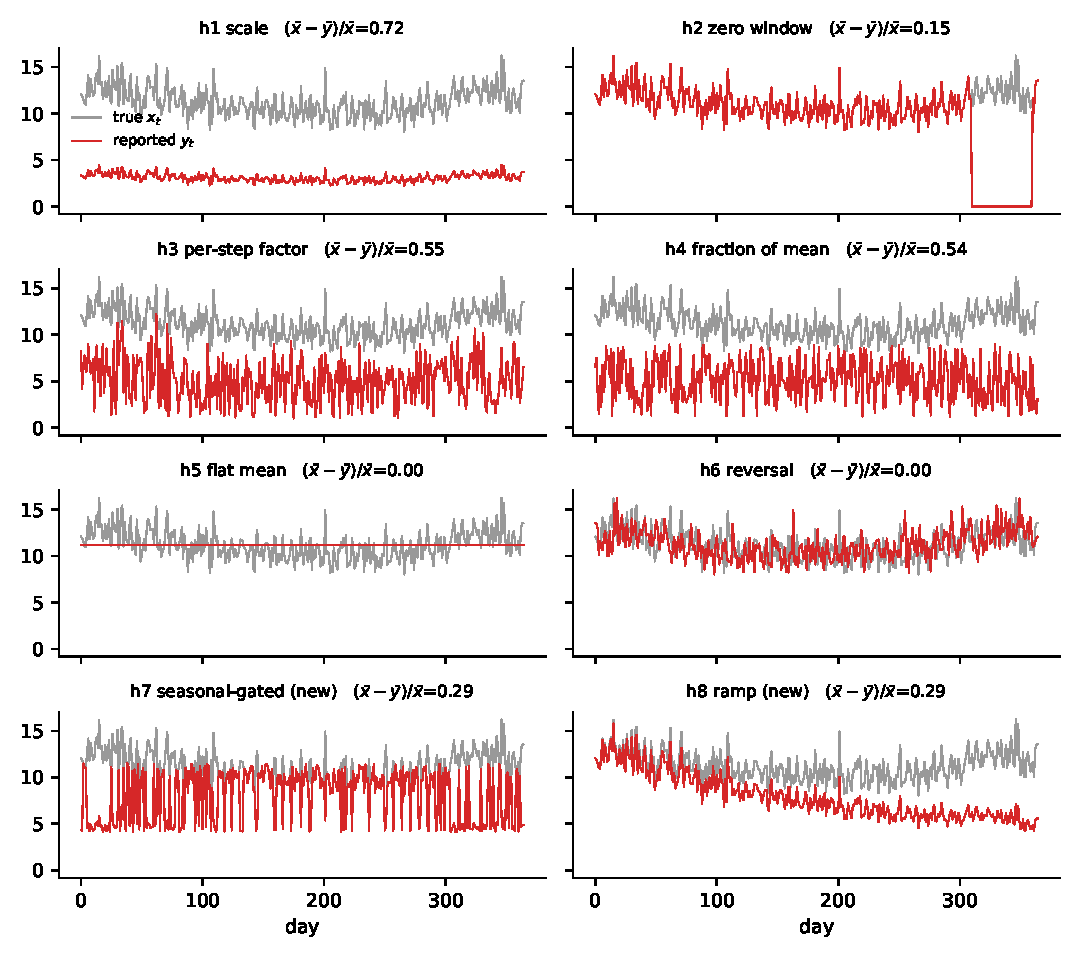
\includegraphics[width=\linewidth]{figs/s2_attacks.pdf}
\caption{The eight attacks applied to one honest residential meter of the seed-0 network. $h_5$ and $h_6$ steal no energy on average (\cref{prop:h56}).}
\label{fig:attacks}
\end{figure}

\subsection{Static attributes}
For each meter: contracted power $=\bar x_i\cdot\mathcal U(\text{archetype range})$ (computed from \emph{true} consumption); meter age $\sim\mathcal N(9,3^2)$ for thieves and $\mathcal N(7,3^2)$ otherwise, clipped to $[0,20]$; alarm count $\sim\mathrm{Poisson}(1.8)$ for thieves and $\mathrm{Poisson}(0.8)$ otherwise; region index near 0.6 on hot and 0.4 on cold feeders; tariff (matching archetype with probability 0.85); archetype one-hot. $D=10$.

\begin{assumption}[Label-dependent static attributes]
\label{as:static}
Meter age and alarm counts are drawn from label-dependent distributions, contracted power is tied to true rather than reported consumption, and region is correlated with theft through hot feeders. This encodes field reports that tampered meters are older and raise more alarms \citep{buzau2019} and that billed energy falls below contracted capacity \citep{terciyanli2017}, but the \emph{strength} of these signals is the author's choice.
\end{assumption}
To quantify how much signal this injects, each attribute was scored alone against the labels (ROC-AUC, no training; seed 0, with the range over seeds 0--4 in brackets): meter age $0.685$ [0.665--0.685]; alarms $0.700$ [0.700--0.732]; contracted power / reported mean $0.817$ [0.806--0.843]; region $0.789$ [0.707--0.789]. Any gain from the static branch on simulated data is bounded by, and partly produced by, this assumption.

\subsection{Technical losses and head readings}
Per feeder, with $d_i\sim\mathcal U(0.3,1)$ a per-customer line factor,
\begin{equation}
\tilde\ell_{f,t}=\sum_{i\in\mathcal C_f}d_i\,x_{i,t}^2+0.3\,\frac{\big(\sum_{i}x_{i,t}\big)^2}{K_f},\qquad
\ell_{f,t}=\lambda_f\tilde\ell_{f,t},\quad \lambda_f=\frac{\tau_f\sum_t\sum_ix_{i,t}}{\sum_t\tilde\ell_{f,t}},\quad \tau_f\sim\mathcal U(0.04,0.09),
\end{equation}
i.e.\ an $I^2R$-type line term plus a transformer copper-loss term, scaled so the annual loss share equals $\tau_f$. Because losses are quadratic in load, the daily loss share varies with demand (0.062--0.106 on feeder 0, \cref{fig:lossfrac}); the model's single $\hat\tau$ is an approximation.

\begin{figure}[htbp]
\centering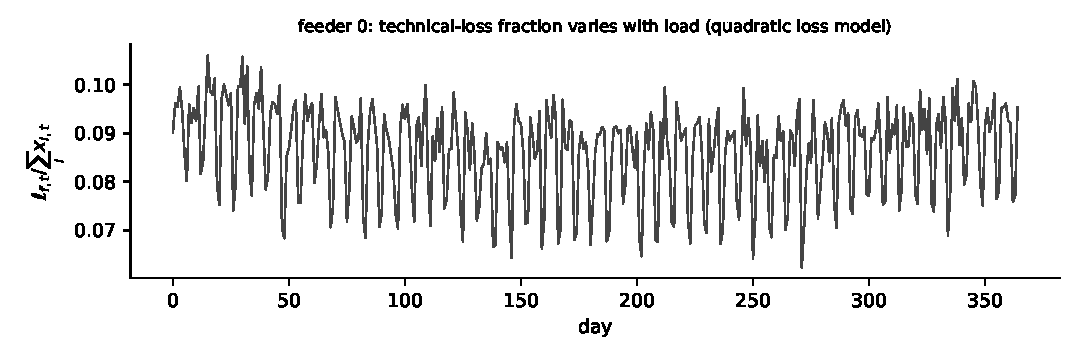
\includegraphics[width=\linewidth]{figs/s4_lossfrac.pdf}
\caption{Daily technical-loss share on one simulated feeder. A constant-share assumption is an approximation even before real-world effects.}
\label{fig:lossfrac}
\end{figure}

\begin{figure}[htbp]
\centering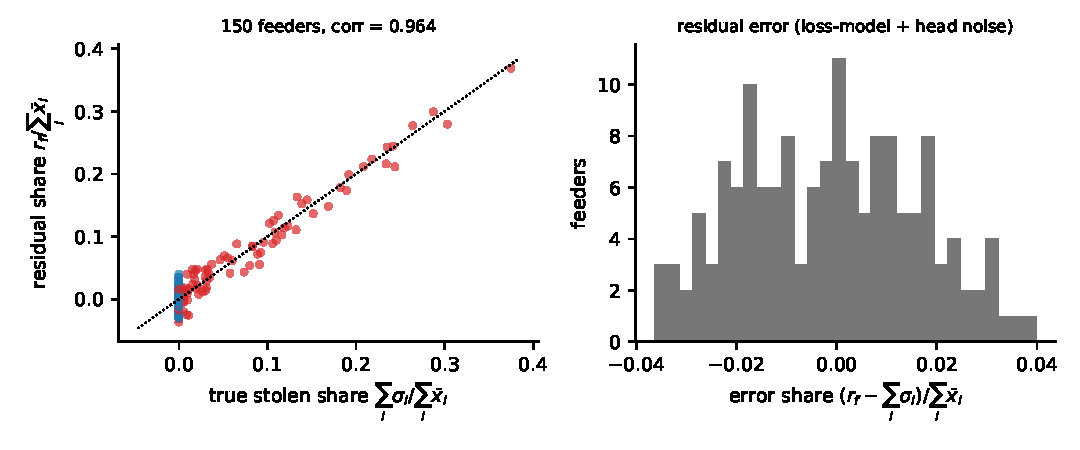
\includegraphics[width=\linewidth]{figs/s3_balance.pdf}
\caption{Left: feeder residual share vs true stolen share for the 150 seed-0 feeders (red: at least one thief). Right: error distribution, s.d.\ $0.0177$, matching the prediction $0.018$ from \cref{prop:residual}.}
\label{fig:balance}
\end{figure}

\begin{figure}[htbp]
\centering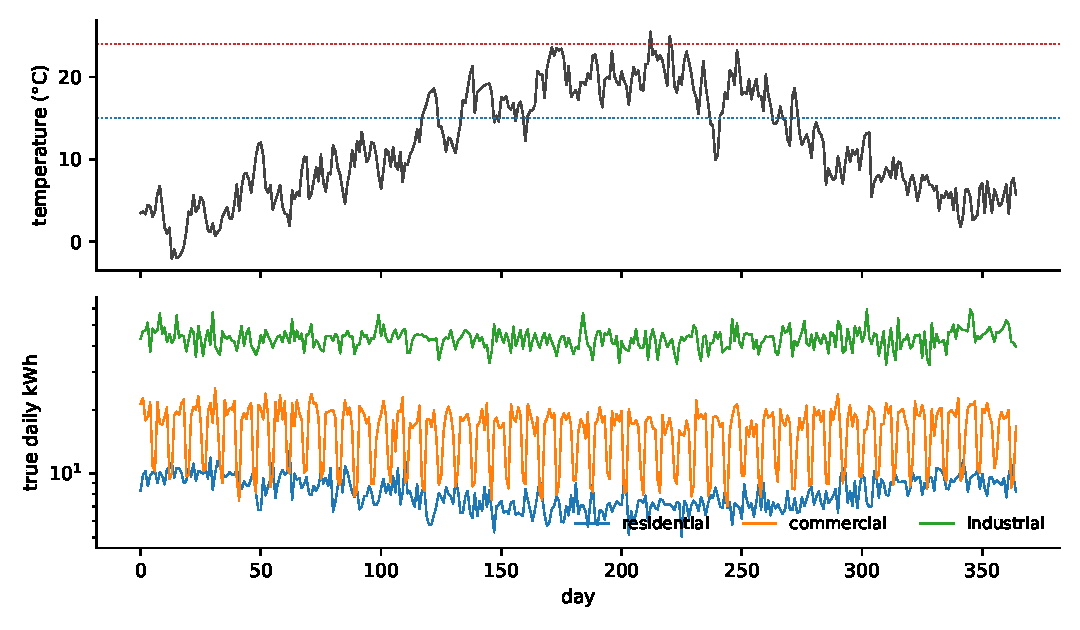
\includegraphics[width=\linewidth]{figs/s1_weather_demand.pdf}
\caption{Simulated temperature (dotted: heating and cooling thresholds) and one true series per archetype (log scale).}
\label{fig:weather}
\end{figure}

\subsection{Second generator for the baselines}
A simpler per-customer generator (\texttt{ntl/data.py}) produces 4{,}000 independent series with a random-phase annual sinusoid (amplitude 0.35), weekend factor $\mathcal U(1.1,1.4)$, log-normal level, Gaussian noise and vacancy gaps; 9\% become thieves under $h_1$--$h_6$. It has no feeders, heads or static attributes and is used only for the baseline comparison.

%=====================================================================
\section{Model: PI-STGAT}
\label{sec:model}
%=====================================================================
\subsection{Input normalisation}
Series are transformed as $\tilde y_{i,t}=(\log(1+y_{i,t})-\mu)/s$ with scalars $\mu,s$ fitted on training-split meters. Static vectors are standardised per column on the training split. Energies entering the conservation term are divided by $u$, the mean head reading of training feeders.

\subsection{Branches}
\paragraph{Temporal.} Two dilated 1-D convolution blocks (32 and 64 channels, kernel 5, dilation 1 and 2; batch norm, ReLU, dropout 0.2) give a receptive field of $1+4\cdot1+4\cdot2=13$ days. Max-pooling by 4 yields $T'=\lfloor T/4\rfloor$ tokens (91 for $T=365$), projected to $d=64$. Multi-head self-attention (4 heads, head dimension 16; no positional encoding) is applied with a residual connection and layer norm:
\begin{equation}
\bm U=\mathrm{LN}\big(\bm V+\mathrm{MHA}(\bm V,\bm V,\bm V)\big),\qquad
\mathrm{head}_j=\mathrm{softmax}\Big(\frac{\bm V\bm W^Q_j(\bm V\bm W^K_j)^\top}{\sqrt{16}}\Big)\bm V\bm W^V_j .
\end{equation}
The readout is $\bm h^{\rm tmp}_i=[\mathrm{mean}_t\bm U;\ \max_t\bm U]\in\R^{128}$.

\paragraph{Static.} $\bm h^{\rm st}_i=\bm W_2\,\mathrm{ReLU}(\bm W_1\bm s_i)$, $\R^D\to\R^{64}\to\R^{32}$.

\paragraph{Fusion.} $\bm h_i=\mathrm{ReLU}(\bm W_f[\bm h^{\rm tmp}_i;\bm h^{\rm st}_i])\in\R^{64}$.

\paragraph{Feeder attention.} Meters of one feeder are padded into a batch row with mask $m\in\{0,1\}^{K_{\max}}$ and updated by masked multi-head attention (padding rows are excluded from the temporal encoder, so they do not reach batch normalisation):
\begin{equation}
\bm h_i\leftarrow\mathrm{LN}\Big(\bm h_i+\sum_{j\in\mathcal C_f}\alpha_{ij}\bm W^V\bm h_j\Big),\qquad
\alpha_{ij}=\frac{\exp(q_i^\top k_j/\sqrt{16})}{\sum_{j'\in\mathcal C_f}\exp(q_i^\top k_{j'}/\sqrt{16})}
\end{equation}
(per head). The graph is the disjoint union of complete graphs, one per transformer; the model uses feeder \emph{membership}, not line distances or electrical topology within the feeder.

\paragraph{Conservation head and classifier.}
\begin{equation}
\hat s_i=\softplus(\bm w_s^\top\bm h_i+b_s)\ge0,\qquad
g_i=\bm w_c^\top[\bm h_i;\hat s_i]+b_c,\qquad \hat p_i=\sig(g_i/t^\star).
\end{equation}
$b_s$ is initialised to $-4$ ($\softplus(-4)\approx0.018$) so the conservation term starts small. Without the physics branch, $\hat s_i\equiv0$ and $g_i=\bm w_c^\top\bm h_i+b_c$.

\paragraph{Size.} Parameter counts printed by the training script: temporal only 39{,}937; + static 44{,}769; + feeder attention 61{,}537; full (simulator, $D=10$) 61{,}603; full on the rehearsal export ($D=3$; the region column is excluded from the inputs on real-format data) 61{,}155. The baseline 1-D CNN has 68{,}545.

\subsection{Training objective}
\begin{equation}
\mathcal L=\mathcal L_{\rm cls}+\lambda\,\mathcal L_{\rm cons},\qquad
\mathcal L_{\rm cons}=\frac1B\sum_{f\in\text{batch}}\Big(\sum_{i\in\mathcal C_f}\hat s_i-\max\big(0,r_f/u\big)\Big)^2,\qquad \lambda=0.5 .
\label{eq:loss}
\end{equation}

\paragraph{Fully labelled case: focal loss} \citep{lin2017focal}, with $p_t=\hat p$ if $z=1$ and $1-\hat p$ otherwise,
\begin{equation}
\mathcal L_{\rm cls}=\frac1{N_b}\sum_i-\alpha_{z_i}(1-p_{t,i})^{\gamma}\log p_{t,i},\qquad \alpha_1=0.75,\ \alpha_0=0.25,\ \gamma=2 .
\end{equation}
The factor $(1-p_t)^\gamma$ down-weights well-classified (mostly honest) examples.

\paragraph{Positive--unlabelled case} (\cref{sec:pu}).

\paragraph{Optimisation.} Adam, learning rate $10^{-3}$, weight decay $10^{-4}$, batches of 16 feeders, 200 epochs in the reported run; the epoch with the highest validation AUPR is kept.

\subsection{Positive--unlabelled learning}
\label{sec:pu}
\begin{assumption}[SCAR]
\label{as:scar}
Confirmed thieves are a uniformly random subset of all thieves (``selected completely at random'' \citep{elkan2008,bekker2020}): $\Prob(\text{confirmed}\mid z=1,\bm o)=c$, constant.
\end{assumption}
Real inspection outcomes violate SCAR, because inspections are targeted; the rehearsal export satisfies it by construction (random 30\% reveal). See \cref{sec:threats}. In simulator PU runs the hidden labels are hidden on the validation split too, so epoch selection, calibration and the threshold use only confirmed labels; the test split keeps full labels for evaluation. The default prior in simulator runs is still the true prevalence, which a utility would not know.

\paragraph{Unbiased risk.} With the sigmoid loss $\ell(g,+1)=\sig(-g)$, $\ell(g,-1)=\sig(g)$, let $p_+$, $p_-$ be the class-conditional feature distributions. Under SCAR the labelled set is a sample of $p_+$ and the unlabelled set a sample of $p_u=\pi_up_++(1-\pi_u)p_-$, where $\pi_u$ is the positive fraction among \emph{unlabelled} meters. Since $(1-\pi_u)\E_-[\ell(g,-1)]=\E_u[\ell(g,-1)]-\pi_u\E_+[\ell(g,-1)]$, the risk with class prior $\pi_u$ can be estimated from labelled and unlabelled data only \citep{kiryo2017}:
\begin{equation}
\widehat R(g)=\hat\pi\,\widehat R_+^{+}+\underbrace{\big(\widehat R_u^{-}-\hat\pi\,\widehat R_+^{-}\big)}_{\widehat R_{\rm neg}},\qquad
\widehat R_+^{\pm}=\tfrac1{|\mathcal P|}\textstyle\sum_{i\in\mathcal P}\sig(\mp g_i),\quad
\widehat R_u^{-}=\tfrac1{|\mathcal U|}\textstyle\sum_{i\in\mathcal U}\sig(g_i).
\end{equation}
\paragraph{Non-negative correction as implemented.} $\widehat R_{\rm neg}$ estimates a non-negative quantity but can become negative under overfitting. In \texttt{ntl/pu.py}, per mini-batch: if $\widehat R_{\rm neg}<0$ the returned loss is $\hat\pi\widehat R_+^+-\widehat R_{\rm neg}$ (so the gradient step raises $\widehat R_{\rm neg}$ back toward zero), else $\hat\pi\widehat R_+^++\widehat R_{\rm neg}$; this is the $\beta=0,\gamma=1$ form of \citet{kiryo2017}.

\paragraph{Which prior.} The code's unlabelled set excludes confirmed meters, so the consistent prior is $\pi_u$, not the overall prevalence $\pi$. If $\rho$ is the observed confirmed fraction,
\begin{equation}
\pi_u=\frac{\pi-\rho}{1-\rho},\qquad c=\rho/\pi .
\label{eq:piu}
\end{equation}

\begin{proposition}[Prior misspecification]
\label{prop:prior}
Under \cref{as:scar}, the population objective $\E[\widehat R]$ with prior $\hat\pi$ equals
\begin{equation}
\E[\widehat R(g)]=(2\hat\pi-\pi_u)\,\E_+\big[\sig(-g)\big]+(1-\pi_u)\,\E_-\big[\sig(g)\big]+(\pi_u-\hat\pi).
\label{eq:effobj}
\end{equation}
If $\hat\pi<\pi_u/2$, the coefficient $a=2\hat\pi-\pi_u$ is negative. Using $\sig(-g)=1-\sig(g)$ the objective becomes $|a|\,\E_+[\sig(g)]+(1-\pi_u)\,\E_-[\sig(g)]+\text{const}$: both classes are driven toward ``honest'', and the population minimiser ($g\to-\infty$ everywhere) flags no meter. Separating the classes is no longer rewarded; any ranking that survives comes only from negatives being pushed down with weight $1-\pi_u$ against $|a|$ for positives.
\end{proposition}
\begin{proof}
$\E_u[\sig(g)]=\pi_u\E_+[\sig(g)]+(1-\pi_u)\E_-[\sig(g)]$, hence $\E[\widehat R]=\hat\pi\E_+\sig(-g)+(\pi_u-\hat\pi)\E_+\sig(g)+(1-\pi_u)\E_-\sig(g)$. The sigmoid loss satisfies $\sig(g)+\sig(-g)=1$, so $\E_+\sig(g)=1-\E_+\sig(-g)$; collect terms. When $\hat\pi$ is small, $\widehat R_{\rm neg}$ stays positive and the non-negative branch is inactive, so \eqref{eq:effobj} is the objective actually optimised.
\end{proof}

\paragraph{Consequence for the default prior.} Setting $\hat\pi=\rho$ (the confirmed-case rate, the only prevalence a utility observes without an audit) makes $a<0$ iff $\rho<\pi_u/2$, i.e.\ $\pi>\rho(3-2\rho)\approx3\rho$; equivalently $c\lesssim 1/3$. In the five rehearsal exports 30\% of thieves were confirmed, $\rho=0.032$--$0.044$ among kept meters and the true prevalence was $0.105$--$0.145$, so \eqref{eq:piu} gives $\pi_u=0.075$--$0.106$ and $a=2\hat\pi-\pi_u\in[-0.018,-0.009]$: negative on every export.

\paragraph{What the proposition does and does not predict.} It describes the population minimiser. A finite network trained for a finite number of epochs need not reach it, and model selection on validation AUPR can keep an early or favourable epoch. The testable consequence is therefore instability during training, not a fixed final outcome. \Cref{sec:rehearsal} reports both: the share of epochs with validation ROC-AUC below 0.5 falls steadily as $\hat\pi$ grows, while final rankings after model selection do not differ consistently between priors. The fall is gradual rather than a jump at $a=0$: at $\hat\pi=0.06$, $a>0$ on every export, yet one export still spent 48\% of its epochs below 0.5. The proposition suggests $\hat\pi\approx\pi_u$ as the consistent choice; the sweep shows no consistent peak there.

\subsection{Physically coherent augmentation}
During training, each honest meter is converted with probability $p$ into a synthetic thief: $y\mapsto\tilde y=A(y)$ for an augmenter $A$, label set to 1, marked as a known positive under PU, and the head reading left unchanged.
\begin{proposition}[Coherence]
\label{prop:aug}
After augmenting honest meter $j$ on feeder $f$, the residual becomes $r_f+\tilde\sigma_j$ with $\tilde\sigma_j=\bar y_j-\bar{\tilde y}_j$, which is exactly the residual \eqref{eq:residid} of a network in which meter $j$ steals $\tilde\sigma_j$.
\end{proposition}
\begin{proof}
True consumption and $\bar H_f$ are unchanged; only $\bar y_j$ in \eqref{eq:resid} changes. For an honest meter $\bar x_j=\bar y_j$, so $\tilde\sigma_j=\bar x_j-\bar{\tilde y}_j$ is its stolen energy.
\end{proof}
Synthetic positives are generated only for training-split feeders, after the feeder-level split, so no synthetic sample is derived from a validation or test meter. Under PU, conversion applies to every unlabelled meter, because a hidden thief cannot be told apart from an honest one, and the cVAE trains on confirmed pairs only.

\subsection{Learned augmenter: conditional VAE over theft masks}
For a theft pair $(x,y)$ define the mask $m_t=\mathrm{clip}(y_t/x_t,0,1)$ (1 where $x_t\le10^{-3}$), downsampled by adaptive average pooling to length 64. The condition is $\bm c=[\text{shape}(x/\bar x)\in\R^{32};\ \log\bar x]$. Encoder $q_\phi(\bm z\mid\bm m,\bm c)=\mathcal N(\bm\mu,\mathrm{diag}\,e^{\bm v})$ with $\bm z\in\R^{16}$; decoder $\hat{\bm m}=\sig(\mathrm{MLP}([\bm z;\bm c]))$. Loss (full batch, Adam $10^{-3}$, 2{,}000 epochs in the reported run):
\begin{equation}
\mathcal L_{\rm VAE}=\|\hat{\bm m}-\bm m\|_2^2/64+\beta\,\mathrm{KL}\big(q_\phi\,\|\,\mathcal N(0,I)\big),\quad
\mathrm{KL}=-\tfrac12\textstyle\sum_{k=1}^{16}\big(1+v_k-\mu_k^2-e^{v_k}\big),\quad\beta=0.01,
\end{equation}
with the reparameterisation $\bm z=\bm\mu+e^{\bm v/2}\odot\bm\epsilon$ \citep{kingma2014,sohn2015}. Sampling: $\bm z\sim\mathcal N(0,I)$, decode, linearly interpolate to length $T$, $\tilde y=\hat m\odot y$.
\begin{proposition}[Support]
\label{prop:cvae}
Every sample satisfies $0<\tilde y_t<y_t$ wherever $y_t>0$, hence $\tilde\sigma>0$. Energy-preserving attacks ($h_5,h_6$) are outside the generator's support.
\end{proposition}
\begin{proof}
Sigmoid outputs lie in $(0,1)$ and linear interpolation of values in $(0,1)$ stays in $(0,1)$. An attack with $\sum_t y_t=\sum_tx_t$ and $y\ne x$ requires $y_t>x_t$ for some $t$, i.e.\ $m_t>1$.
\end{proof}
Training pairs require the true series. In simulation they are known; on real data they would be the post-inspection corrected consumption of confirmed cases (not yet available, so the learned augmenter is disabled in real mode).

\subsection{Self-supervised pretraining}
The temporal encoder is pretrained on training-split series by masked-span reconstruction: random spans of 5--21 days are hidden until 30\% of each series is covered, hidden values are set to 0 (the normalised mean), and a per-token linear decoder ($\R^{64}\to\R^4$) reconstructs the series; the loss is mean squared error on hidden positions only (Adam $10^{-3}$, weight decay $10^{-5}$, batch 256, 50 epochs in the reported run). Weights are then copied into the temporal branch. This follows masked autoencoding \citep{he2022mae}; spans are used because single missing days are trivially interpolated.

\subsection{Calibration, threshold and outputs}
\label{sec:calib}
A temperature $t^\star=\arg\min_{t\in[0.5,10]}\mathrm{BCE}(\sig(g/t),z)$ is fitted on the validation split by L-BFGS \citep{guo2017}. Because $g\mapsto g/t$ is monotone, AUPR, ROC-AUC, P@$k$, R@$k$ and ER@$k$ are unchanged by calibration. The decision threshold maximises F1 on calibrated validation probabilities and is used only for flag rates and F1. In the fully labelled simulator runs the fitted temperature was 0.50--0.96 and often at the lower bound $0.5$ (the optimiser would have sharpened further); in PU simulator runs it was 1.4--3.0, and in the rehearsal with $\hat\pi=0.13$ it was 1.24--2.77. On real-format data calibration uses confirmed labels, so $\hat p$ estimates the probability of being a \emph{confirmed} case, which is lower than the probability of theft.

The ranking export contains $\hat p_i$, $\hat s_i u$ (estimated kWh/day) and the product $\hat p_i\hat s_i$.

\begin{remark}[Ranking key]
By \cref{lem:keys}(b) the energy-optimal key is $\E[\sigma\mid\bm o]$. The conservation head is trained to make $\sum_i\hat s_i$ match the \emph{unconditional} feeder theft, so $\hat s_i$ targets $\E[\sigma_i\mid\cdot]$ itself, which already contains the theft probability. Ranking by $\hat p_i\hat s_i$ then counts the probability twice. Ranking by $\hat s_i$ alone is the key the theory suggests; it has not been evaluated. Empirically $\hat p\hat s$ captured slightly more stolen energy than $\hat p$ (\cref{sec:er}).
\end{remark}

%=====================================================================
\section{Baselines}
\label{sec:baselines}
%=====================================================================
\textbf{1-D CNN.} Three dilated convolution blocks (32/64/128 channels, kernel 5, dilations 1/2/4), mean+max pooling, MLP head; focal loss; on-the-fly $h_1$--$h_6$ augmentation with $p=0.15$; 150 epochs in the reported run, batch 128; customer-level stratified 70/15/15 split.

\textbf{XGBoost} \citep{buzau2019}. Ten per-customer features: mean, s.d., min, max, median, zero-day fraction, skewness, kurtosis, coefficient of variation, lag-1 autocorrelation; 400 trees, depth 5, learning rate 0.05, subsampling 0.9, \texttt{scale\_pos\_weight} $=n_-/n_+$; no augmentation; same split protocol as the CNN.

%=====================================================================
\section{Evaluation protocol}
%=====================================================================
\textbf{Splits.} PI-STGAT splits whole feeders 70/15/15 (train/validation/test), so no test meter's neighbours appear in training. Baselines split customers.

\textbf{Metrics.} AUPR is average precision, $\mathrm{AP}=\sum_n(R_n-R_{n-1})P_n$; ROC-AUC equals $\Prob(g_+>g_-)$ \citep{hanley1982}. AUPR is preferred under imbalance \citep{davis2006,saito2015}, but it depends on prevalence: at a fixed operating point,
\begin{equation}
\mathrm{precision}=\frac{\pi\,\mathrm{TPR}}{\pi\,\mathrm{TPR}+(1-\pi)\,\mathrm{FPR}},
\end{equation}
and a random score has $\E[\mathrm{AP}]\approx\pi$. AUPR values are comparable only at equal prevalence; ROC-AUC is prevalence-invariant. Recall at a budget is capped by prevalence:
\begin{equation}
\mathrm{R@}k\le\min\big(1,\,k/(N\pi)\big),
\end{equation}
so with feeder-clustered theft and a 15\% feeder test split, R@10\% varies strongly between seeds through the test prevalence alone.

\textbf{Evaluation under PU labels.} On real data only confirmed labels exist.
\begin{proposition}[Confirmed-only evaluation]
\label{prop:pueval}
Under \cref{as:scar} with labelling frequency $c$ on the evaluation set, for every threshold $\E[\mathrm{TP}_{\rm vis}]=c\,\mathrm{TP}$ while the number flagged is unchanged, so $\E[\mathrm{precision}_{\rm vis}]=c\cdot\mathrm{precision}$ and $\E[\mathrm{recall}_{\rm vis}]=\mathrm{recall}$. Hence $\mathrm{AP}_{\rm vis}\approx c\cdot\mathrm{AP}_{\rm true}$ (in expectation, for large samples), and confirmed-only AUPR understates true AUPR by a factor of about $1/c$. For ROC-AUC, $\mathrm{AUC}_{\rm vis}\approx\pi_u\cdot\tfrac12+(1-\pi_u)\mathrm{AUC}_{\rm true}$.
\end{proposition}
\begin{proof}
Each true positive is visible independently with probability $c$; AP integrates precision over recall. For ROC, a confirmed positive is compared against an unlabelled meter that is a hidden positive with probability $\pi_u$ (coin flip on average) and a negative otherwise.
\end{proof}

\textbf{Seeds.} The seed controls both the simulated network and the model initialisation, so seed-to-seed spread includes data variation.

%=====================================================================
\section{Results}
%=====================================================================
\begin{table}[htbp]
\centering\small
\begin{tabular}{@{}p{3.6cm}p{8.6cm}p{2.4cm}@{}}
\toprule
Experiment & Data & Runs\\
\midrule
Baselines & per-customer generator, 4{,}000 meters, $T=365$, 9.2\% test prevalence & 5 seeds each\\
Baseline CNN on simulator & each seed's simulator network flattened to per-customer rows (2{,}973--3{,}249 meters) & 5 seeds\\
Ablation (4 configurations) & simulator, 150 feeders, $T=365$, prevalence 0.111--0.174 & 5 seeds each\\
Variants of the full model & SSL + augmentation; positional code; region removed; label-free age and alarms; PU with 30\% revealed, with and without SSL & 5 seeds each\\
Unseen-attack experiment & train 2{,}099--2{,}326 meters, $h_1$--$h_4$ only, 2.9--3.7\%; test on an independent network of 1{,}098--1{,}245 meters, $h_1$--$h_8$, 9.5--17.4\% & 5 seeds $\times$ 4\\
Deployment rehearsal & one defective export per seed, 60 feeders, $T=240$; 1{,}061--1{,}291 meters used; 5 priors & 5 exports $\times$ 5 priors\\
\bottomrule
\end{tabular}
\caption{Experiments in the reported run. Counts are those printed by the scripts. The seed fixes the network, the split and the initialisation, so seed-to-seed spread includes data variation.}
\label{tab:exp}
\end{table}

\begin{figure}[htbp]
\centering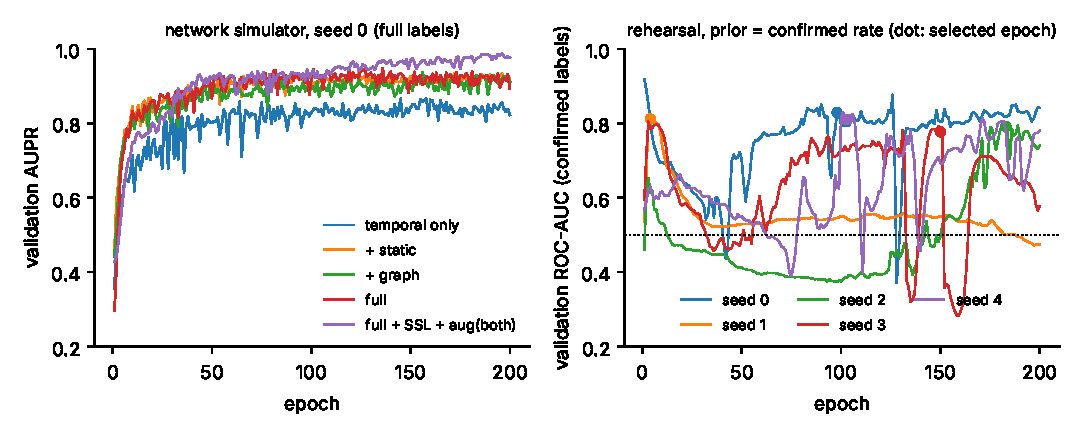
\includegraphics[width=\linewidth]{figs/s5_curves.pdf}
\caption{Validation curves from the training logs. Left: simulator, seed 0, full labels; all configurations are still improving slowly after 100 epochs. Right: rehearsal with the PU prior set to the confirmed rate, one line per export; dots mark the selected epoch. Validation ROC-AUC (against confirmed labels) spends long stretches below 0.5 on several exports.}
\label{fig:curves}
\end{figure}

\subsection{Baselines and the per-customer comparison}
\begin{figure}[htbp]
\centering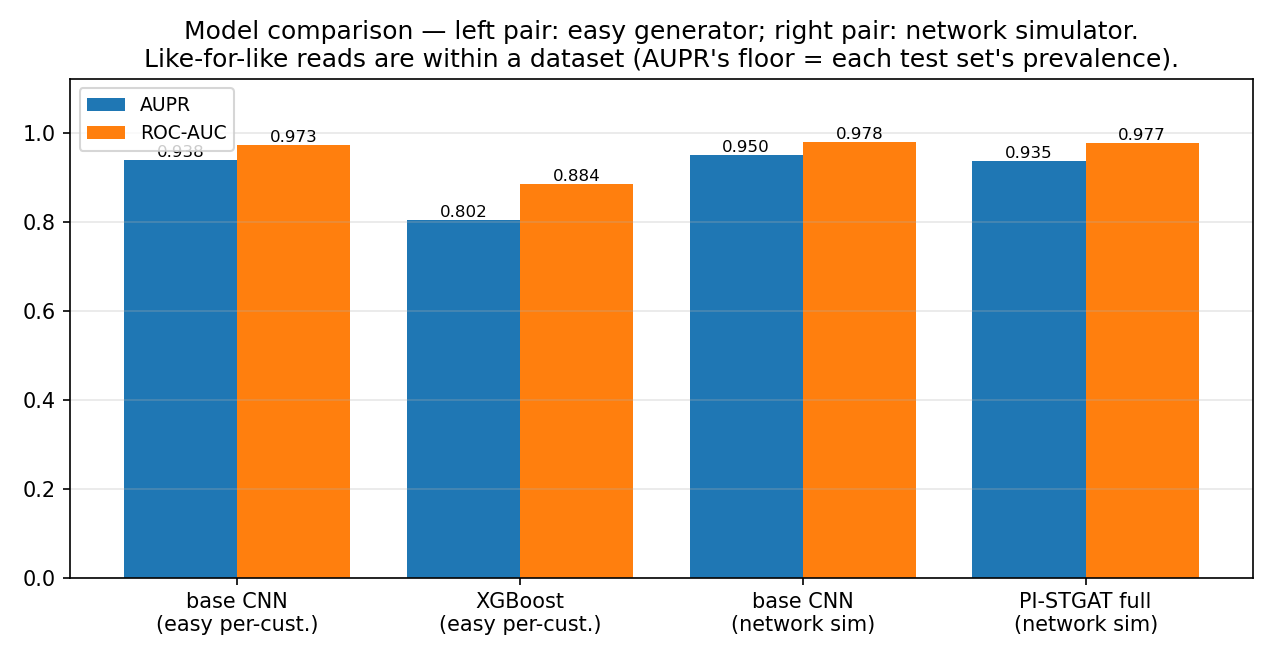
\includegraphics[width=0.9\linewidth]{figs/fig1_model_comparison.png}
\caption{Model comparison, mean of 5 seeds. Left pair: per-customer generator. Right pair: network simulator. Bars within a pair share a dataset but not necessarily a split (see text).}
\label{fig:f1}
\end{figure}
On the per-customer generator the CNN reaches AUPR $0.938\pm0.024$ / ROC-AUC $0.973\pm0.014$ and XGBoost $0.802\pm0.034$ / $0.884\pm0.016$ (mean $\pm$ s.d.\ over 5 seeds, prevalence 0.092). On the simulator the CNN, given each meter's reported series only, reaches $0.950\pm0.021$ / $0.978\pm0.010$; full PI-STGAT reaches $0.935\pm0.028$ / $0.977\pm0.010$.

\textbf{This comparison does not show an advantage for PI-STGAT.} It is also not controlled. The CNN uses a customer-stratified split, so meters from one feeder fall into both training and test, while PI-STGAT holds out whole feeders; the CNN is trained with $h_1$--$h_6$ augmentation, which matches six of the eight test attacks, while the ablation configurations use none. Test prevalence is similar on average (0.136 for the CNN, 0.138 for PI-STGAT). The PI-STGAT variant trained with augmentation (and SSL) reaches $0.969\pm0.009$ / $0.984\pm0.007$, above the CNN, but again under a different split. A comparison on the same feeder split with the same augmentation is needed before any architectural claim (\cref{sec:next}).

\subsection{Ablation and variants}
\label{sec:abl}
\begin{figure}[htbp]
\centering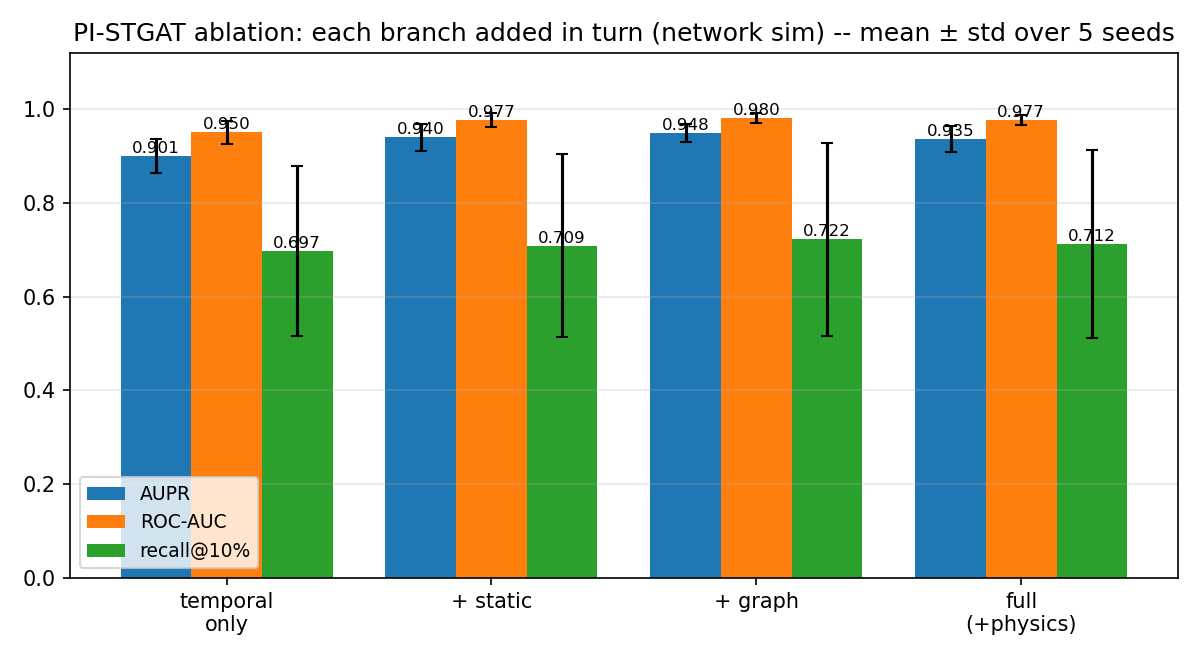
\includegraphics[width=0.9\linewidth]{figs/fig2_ablation.png}
\caption{Ablation, mean $\pm$ s.d.\ over 5 seeds.}
\label{fig:f2}
\end{figure}
\begin{table}[htbp]
\centering\small
\begin{tabular}{@{}lccc@{}}
\toprule
Configuration (5 seeds) & AUPR & ROC-AUC & R@10\%\\
\midrule
Temporal only & $0.901\pm0.037$ & $0.950\pm0.026$ & $0.697\pm0.181$\\
+ static & $0.940\pm0.029$ & $0.977\pm0.014$ & $0.709\pm0.195$\\
+ feeder attention & $0.948\pm0.019$ & $0.980\pm0.011$ & $0.722\pm0.205$\\
+ physics (full) & $0.935\pm0.028$ & $0.977\pm0.010$ & $0.712\pm0.201$\\
\midrule
Full + SSL + augmentation & $0.969\pm0.009$ & $0.984\pm0.007$ & $0.731\pm0.214$\\
Full + positional code & $0.971\pm0.007$ & $0.988\pm0.007$ & $0.722\pm0.205$\\
Full, region input removed & $0.939\pm0.026$ & $0.978\pm0.012$ & $0.722\pm0.205$\\
+ static, age and alarms label-free & $0.950\pm0.013$ & $0.980\pm0.003$ & $0.713\pm0.198$\\
Full, age and alarms label-free & $0.945\pm0.022$ & $0.981\pm0.008$ & $0.715\pm0.201$\\
\bottomrule
\end{tabular}
\caption{Ablation and variants, mean $\pm$ s.d.\ over 5 seeds.}
\label{tab:abl}
\end{table}

Because each seed fixes the network and split, configurations can be compared seed by seed. \Cref{tab:paired} lists the paired AUPR differences.
\begin{table}[htbp]
\centering\small
\begin{tabular}{@{}lccc@{}}
\toprule
Comparison & per-seed AUPR difference (seeds 0--4) & mean & higher on\\
\midrule
+ static $-$ temporal & $+0.028, +0.027, +0.069, +0.027, +0.046$ & $+0.039$ & 5/5\\
+ attention $-$ + static & $+0.019, -0.006, -0.007, +0.001, +0.035$ & $+0.008$ & 3/5\\
full $-$ + attention & $-0.021, -0.033, -0.002, +0.001, -0.010$ & $-0.013$ & 1/5\\
full + SSL + aug $-$ full & $+0.021, +0.070, +0.022, +0.014, +0.042$ & $+0.034$ & 5/5\\
full + positional $-$ full & $+0.022, +0.074, +0.016, +0.003, +0.064$ & $+0.036$ & 5/5\\
full + positional $-$ full + SSL + aug & $+0.001, +0.004, -0.006, -0.011, +0.022$ & $+0.002$ & 3/5\\
full, region removed $-$ full & $+0.014, +0.003, -0.011, -0.002, +0.015$ & $+0.004$ & 3/5\\
+ static label-free $-$ temporal & $+0.042, +0.039, +0.053, +0.022, +0.089$ & $+0.049$ & 5/5\\
\bottomrule
\end{tabular}
\caption{Paired per-seed AUPR differences. Five seeds give little power; ``5/5'' is the strongest pattern five seeds can show, not a significance test.}
\label{tab:paired}
\end{table}
\begin{itemize}
\item \textbf{Static attributes} raise AUPR on every seed (+0.039). The gain does not depend on the label-dependent meter age and alarm counts: with both redrawn independently of theft on the same networks, the gain over temporal-only is still positive on every seed (+0.049). It therefore comes from contracted power and region, which also carry theft signal by construction (\cref{as:static}).
\item \textbf{Feeder attention} is not separable from noise (3/5).
\item \textbf{The physics branch} lowers AUPR slightly on four of five seeds ($-0.013$). This is consistent with \cref{prop:rank}: the conservation term fixes feeder totals, not the within-feeder ranking that AUPR measures. Its value is the energy estimate $\hat s$ (\cref{sec:er}).
\item \textbf{A positional code} in the temporal encoder and \textbf{SSL with combined augmentation} each raise AUPR on every seed, by about 0.035, and end within 0.002 of each other. The SSL + augmentation run does not separate the two ingredients.
\item \textbf{R@10\%} has s.d.\ 0.18--0.21 in every configuration. Test prevalence ranges from 0.057 to 0.216 across seeds and R@$k$ is capped at $k/(N\pi)$, so this spread comes mostly from the splits.
\end{itemize}

\subsection{Per-attack recall}
\begin{figure}[htbp]
\centering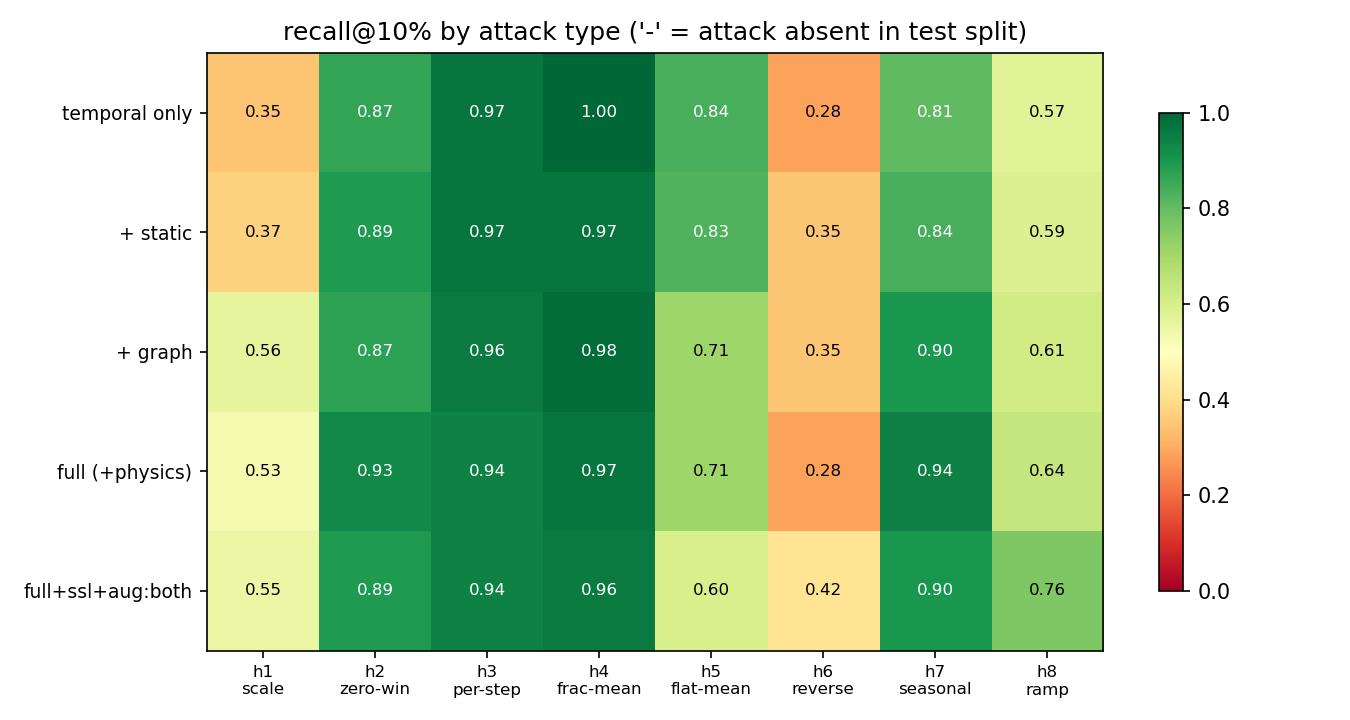
\includegraphics[width=0.9\linewidth]{figs/fig3_attack_recall.png}
\caption{Recall@10\% by attack type, mean of 5 seeds.}
\label{fig:f3}
\end{figure}
Per-step attacks $h_3$, $h_4$ and the zero window $h_2$ are found at 0.87--1.00 in every configuration. Uniform scaling $h_1$ rises from 0.35 (temporal only) to 0.53--0.56 once feeder attention or physics is added. The new seasonal attack $h_7$ is found at 0.81--0.94 and the ramp $h_8$ at 0.58--0.76. Energy-preserving reversal $h_6$ stays lowest, 0.28--0.42 (0.48 with the positional code); flat-mean $h_5$, also energy-preserving, is found at 0.60--0.84 because it removes variance, which permutation-invariant statistics detect.

\textbf{Sample size.} The test splits of the five seeds together contain 29--50 instances of each attack (for $h_6$: 6, 12, 6, 6, 6 per seed). Differences between cells of about 0.1 are within noise.

\subsection{Energy recovery}
\label{sec:er}
\begin{figure}[htbp]
\centering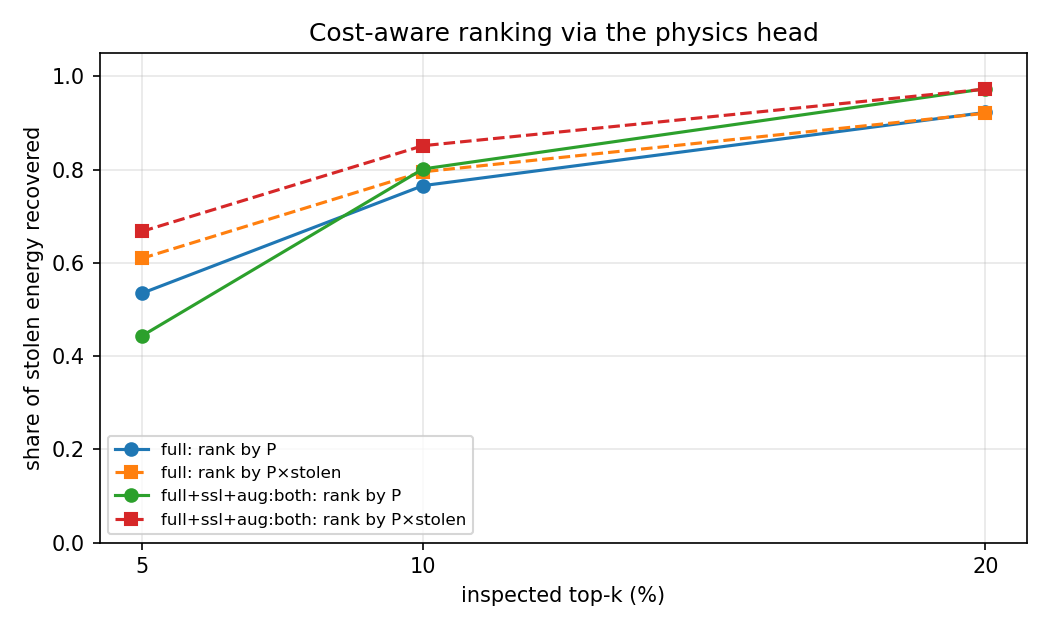
\includegraphics[width=0.75\linewidth]{figs/fig4_energy_recovery.png}
\caption{Share of stolen energy in the inspected top-$k$, mean of 5 seeds.}
\label{fig:f4}
\end{figure}
For the full model, inspecting the top 5\%, 10\% and 20\% recovers 0.54, 0.77 and 0.92 of stolen energy when ranked by $\hat p$, and 0.61, 0.80 and 0.92 when ranked by $\hat p\hat s$. With SSL and augmentation the cost-aware ranking recovers 0.67, 0.85 and 0.97. The 5\% value varies strongly between seeds (0.22--0.99 for the full model ranked by $\hat p$), so only multi-seed values should be quoted. Configurations without the physics branch have $\hat s\equiv0$, so their $\hat p\hat s$ ranking is meaningless.

\subsection{Regional audit}
\begin{figure}[htbp]
\centering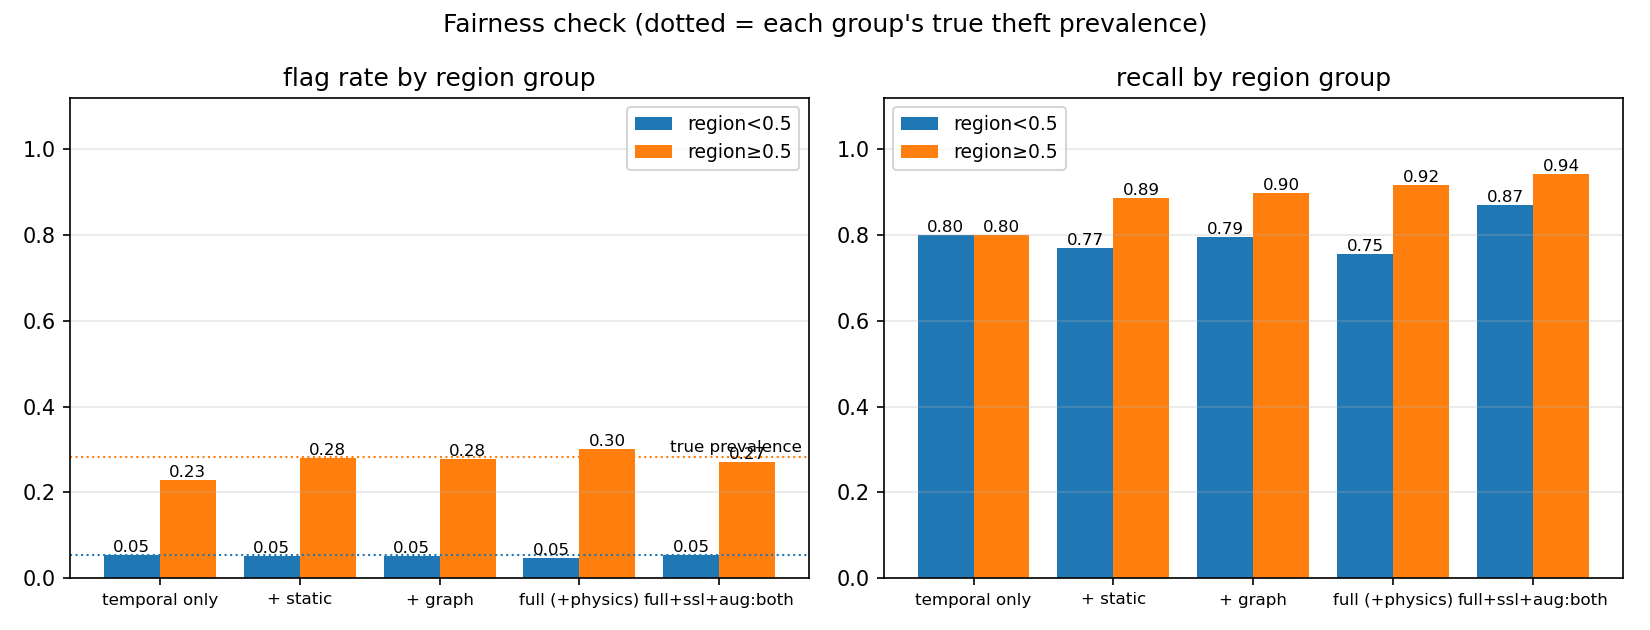
\includegraphics[width=\linewidth]{figs/fig5_fairness.png}
\caption{Flag rate and recall by region group, mean of 5 seeds. Dotted: group prevalence.}
\label{fig:f5}
\end{figure}
Group prevalence is 0.054 (low-region) and 0.283 (high-region). Flag rates follow prevalence: 0.05 in the low group for every configuration, and 0.23--0.30 in the high group. Recall at the operating threshold is balanced for the temporal-only model (0.80 vs 0.80) and becomes unbalanced when static attributes enter (full model 0.76 vs 0.92). Region is itself an input correlated with theft (ROC-AUC 0.71--0.79 alone). Removing it narrows the gap only from 0.16 to 0.13. The two strongest models narrow it more, by raising low-group recall: 0.85 vs 0.93 with the positional code, 0.87 vs 0.94 with SSL and augmentation.

\subsection{Augmentation and attacks withheld from training}
\begin{figure}[htbp]
\centering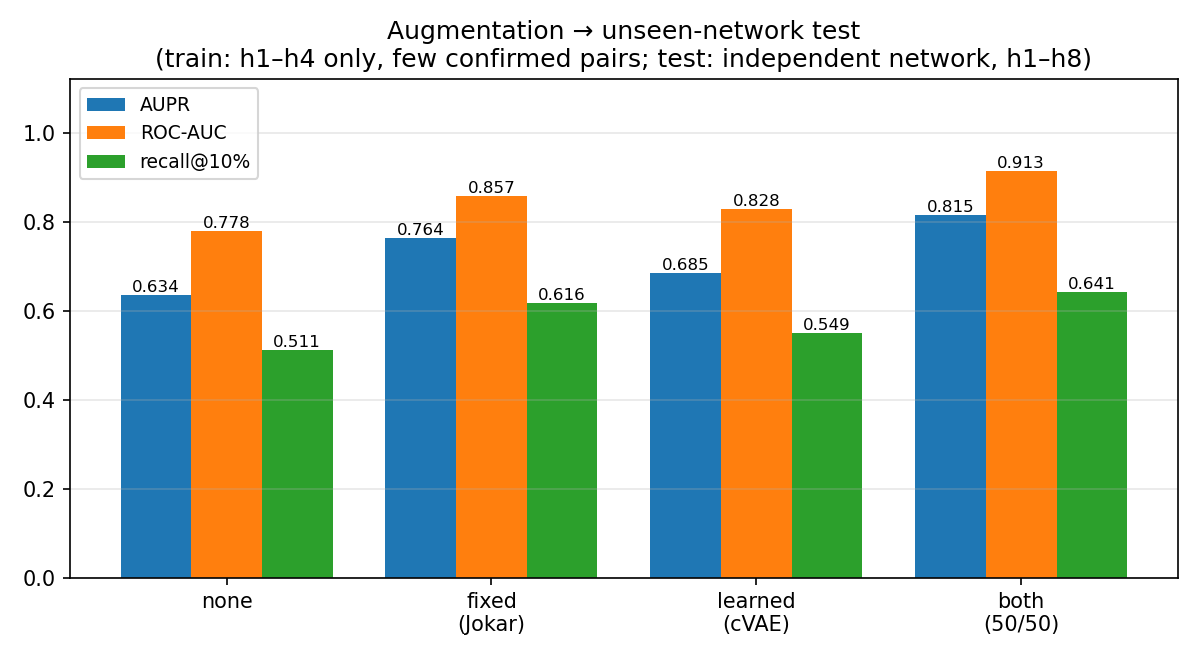
\includegraphics[width=0.85\linewidth]{figs/fig6_augmentation.png}
\caption{Temporal-only model trained on $h_1$--$h_4$ (38--50 confirmed pairs for the cVAE), tested on an independent network with all eight attacks. Mean of 5 seeds.}
\label{fig:f6}
\end{figure}
\begin{figure}[htbp]
\centering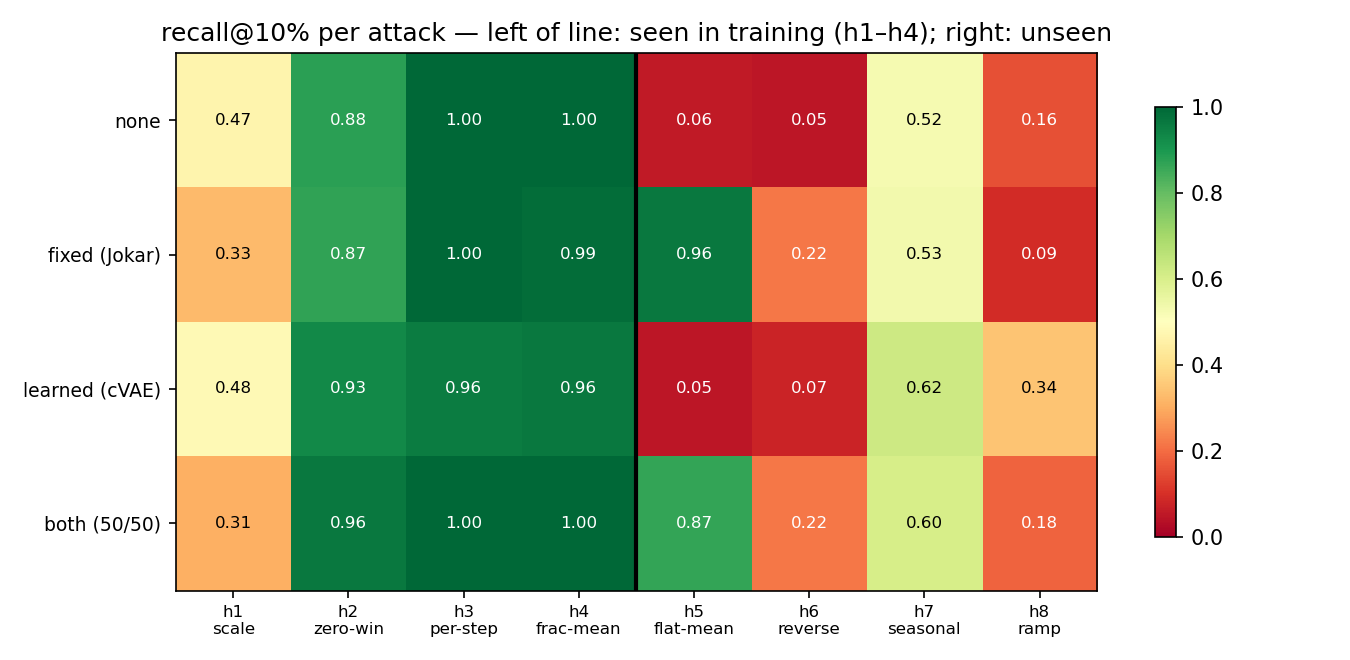
\includegraphics[width=0.9\linewidth]{figs/fig7_aug_per_attack.png}
\caption{Per-attack recall@10\% for the same experiment, mean of 5 seeds.}
\label{fig:f7}
\end{figure}
Mean AUPR / ROC-AUC over 5 seeds: no augmentation $0.634$ / $0.778$; fixed functions $0.764$ / $0.857$; learned cVAE $0.685$ / $0.828$; both $0.815$ / $0.913$. Paired against no augmentation, AUPR is higher on 5/5 seeds for both and for the fixed functions, and on 4/5 for the cVAE. The combined augmenter has higher AUPR than the fixed functions alone on 3/5 seeds.

The per-attack pattern matches \cref{prop:cvae}:
\begin{itemize}
\item \textbf{$h_8$ ramp} is unseen by every variant and is a multiplicative under-reporting mask, inside the cVAE's support. The cVAE raises its recall on all five seeds (mean $0.16\to0.34$); the fixed functions never raise it (0.09).
\item \textbf{$h_5$ and $h_6$} are energy-preserving, outside the cVAE's support. The cVAE leaves $h_5$ unchanged (0.06 to 0.05); the fixed functions, which contain $h_5$ and $h_6$ by hand, raise $h_5$ to 0.96 and $h_6$ from 0.05 to 0.22. They are not unseen for that variant.
\item \textbf{$h_7$} (unseen) moves 0.52 / 0.53 / 0.62 / 0.60 (none / fixed / learned / both) with seed s.d.\ 0.13--0.26; no conclusion.
\item \textbf{$h_1$} falls from 0.47 to 0.33 with the fixed functions and to 0.31 with both (lower on 4/5 seeds), so fixed augmentation trades $h_1$ for $h_5$.
\end{itemize}

\subsection{Deployment rehearsal}
\label{sec:rehearsal}
\paragraph{Exports.} \texttt{make\_fake\_export.py} turns each seed's 60-feeder, 240-day simulated network into the CSV files a utility would provide, with defects injected: 10\% of meters with 3--20-day gaps (about 30\% of the missing readings exported as blank kWh rows), 5\% late joiners, 1\% dead meters, 1\% meters missing from the topology file, 1\% assigned to the wrong transformer, 1.5 kWh/day of unmetered load on every head, and 1\% head noise. Thirty percent of thieves, chosen at random, go into the label file; truth is written separately and used only for evaluation.

\paragraph{Ingestion diagnostics} (printed by the loader for the five exports): 1{,}072--1{,}304 meters kept, 35--39 dropped for coverage below 80\%; 11--13 unmapped meters dropped, carrying 0.6--1.3\% of metered load (the loader warns that this load stays in the residuals); 1--2 feeders per export flagged for negative residual (topology or CT errors) and one feeder in one export for residual above 40\%; technical-loss estimate $\hat\tau=0.061$--$0.074$; confirmed rate $\rho=0.032$--$0.044$; true prevalence 0.105--0.145.

\paragraph{Evaluation set.} ``Out-of-sample'' meters in the ranking file include the validation feeders, whose confirmed labels selected the training epoch. All rehearsal numbers below therefore use the 9 test feeders of each export only: 901 meters in total, 142 thieves (base rate 0.158), 40 of them confirmed.

\begin{figure}[htbp]
\centering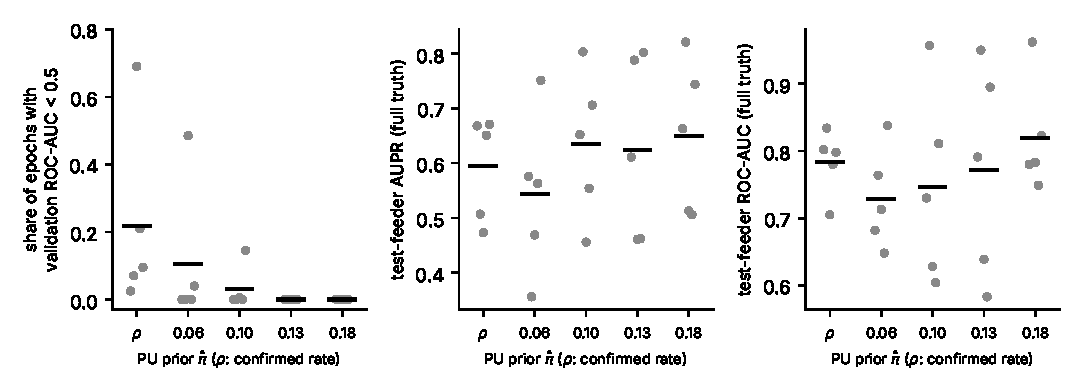
\includegraphics[width=\linewidth]{figs/s6_prior_sweep.pdf}
\caption{Prior sweep over five exports (grey: one export; black: mean). Left: share of training epochs with validation ROC-AUC below 0.5. Middle and right: AUPR and ROC-AUC on test feeders against the full truth, after model selection.}
\label{fig:sweep}
\end{figure}
\begin{table}[htbp]
\centering\small
\setlength{\tabcolsep}{3.5pt}
\begin{tabular}{@{}lccccc@{}}
\toprule
$\hat\pi$ & $\rho$ & 0.06 & 0.10 & 0.13 & 0.18\\
\midrule
Epochs, val.\ ROC $<0.5$ & $0.22\pm0.27$ & $0.10\pm0.21$ & $0.03\pm0.06$ & $0$ & $0$\\
Test AUPR vs truth & $0.59\pm0.10$ & $0.54\pm0.15$ & $0.63\pm0.13$ & $0.63\pm0.17$ & $0.65\pm0.14$\\
Test ROC-AUC vs truth & $0.78\pm0.05$ & $0.73\pm0.07$ & $0.75\pm0.14$ & $0.77\pm0.16$ & $0.82\pm0.08$\\
Hit rate, top 5\% & 36/45 = 0.80 & 34/45 = 0.76 & 42/45 = 0.93 & 39/45 = 0.87 & 38/45 = 0.84\\
\quad Wilson 95\% & [0.66, 0.89] & [0.61, 0.86] & [0.82, 0.98] & [0.74, 0.94] & [0.71, 0.92]\\
Hit rate, top 10\% & 62/90 = 0.69 & 51/90 = 0.57 & 60/90 = 0.67 & 60/90 = 0.67 & 63/90 = 0.70\\
\bottomrule
\end{tabular}
\caption{Prior sweep, test feeders only, mean $\pm$ s.d.\ over five exports; hit rates pooled over the five test sets (base rate 142/901 = 0.158, Wilson 95\% [0.135, 0.183]). $\rho$ is each export's confirmed rate, 0.032--0.044.}
\label{tab:sweep}
\end{table}

\paragraph{Ranking quality.} With any prior, the top 5\% of each test set contains 76--93\% thieves against a base rate of 16\%, and the top 10\% contains 57--70\%. Differences between priors are within the export-to-export spread; no prior is consistently best.

\paragraph{Training stability.} With the confirmed-rate prior ($a<0$ on every export), validation ROC-AUC fell below 0.5 for 2.5--69\% of epochs depending on the export (\cref{fig:curves}); at $\hat\pi\ge0.13$ it never did. The share falls monotonically on average as $\hat\pi$ increases, which is the instability \cref{prop:prior} predicts. Selecting the best validation epoch recovered usable models in every case: at the operating threshold the confirmed-rate runs had flag rates of 0.02--0.39 across the two region groups, not zero. An earlier version of this report, using 20 training epochs, observed a flag rate of zero with this prior; that was not reproduced at 200 epochs.

\paragraph{The understatement factor.} \Cref{prop:pueval} predicts $\mathrm{AP}_{\rm true}/\mathrm{AP}_{\rm vis}\approx1/c$. Over the 25 test-feeder evaluations (5 exports $\times$ 5 priors) the observed ratio has mean 3.5 (median 3.3, range 1.2--8.3); the predicted $1/c$ has mean 3.7 (median 3.8). The ratio is close to the prediction on average but varies widely in single evaluations, which involve 4--10 confirmed thieves each. On a real utility, where only confirmed labels exist, confirmed-only AUPR should be read as roughly a third of the true value at a 30\% confirmation rate, with a wide margin.

\begin{figure}[htbp]
\centering
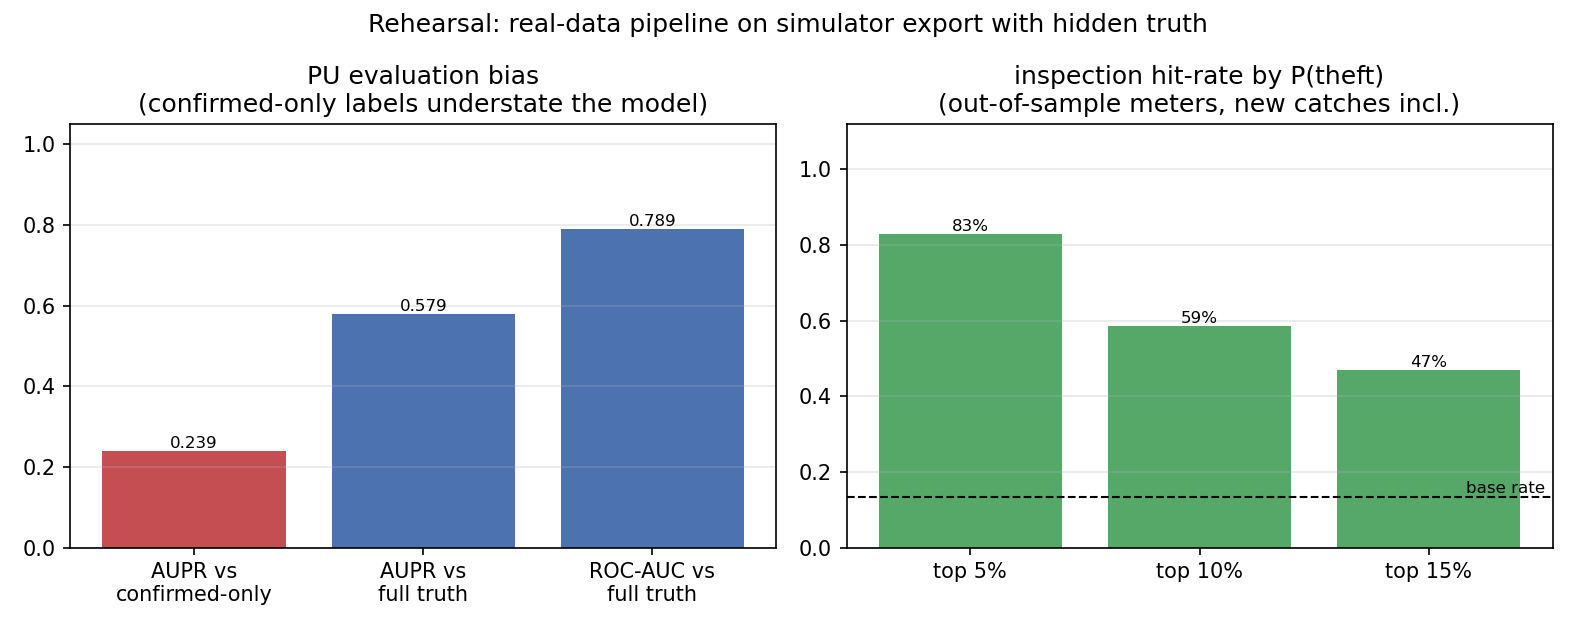
\includegraphics[width=0.82\linewidth]{figs/fig8_prior_default.png}\\[0.5em]
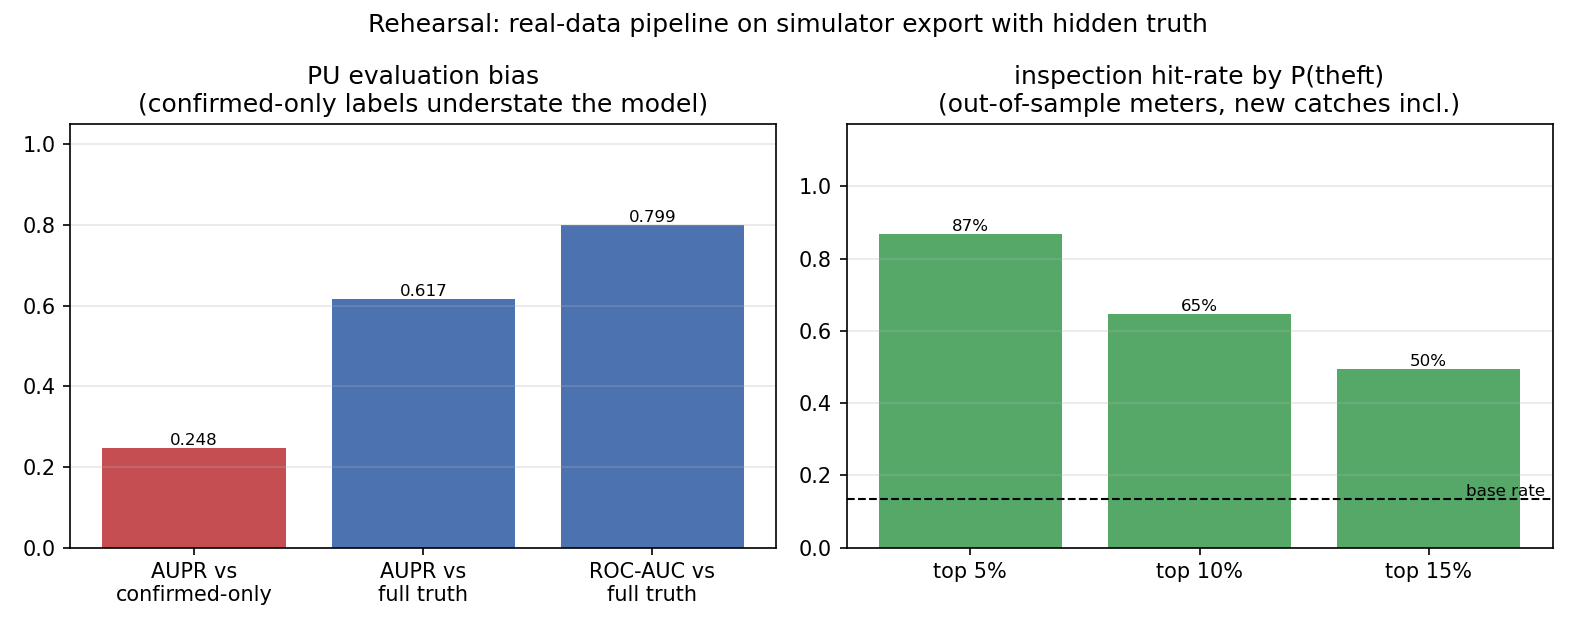
\includegraphics[width=0.82\linewidth]{figs/fig8_rehearsal.png}
\caption{Rehearsal on out-of-sample meters (validation and test feeders), mean of 5 exports. Top: confirmed-rate prior. Bottom: $\hat\pi=0.13$. Because validation feeders selected the epoch, these values are optimistic; \cref{tab:sweep} uses test feeders only.}
\label{fig:f8}
\end{figure}

\paragraph{SSL under scarce labels.} On the simulator with 30\% of thieves revealed (hidden on training and validation, full model), SSL gave test AUPR $0.732\pm0.067$ against $0.657\pm0.125$ without it, and ROC-AUC $0.894$ against $0.857$. Per seed, AUPR was higher with SSL on three seeds (+0.18, +0.22, +0.12) and lower on two ($-0.14$, $-0.02$). The mean favours SSL but five seeds do not settle it.

%=====================================================================
\section{Discussion}
%=====================================================================
\paragraph{What the evidence supports.}
\begin{itemize}
\item On this simulator, ranking quality is high (AUPR 0.94--0.97, ROC-AUC 0.98--0.99 for the better configurations, five seeds). Static attributes, a positional code, and SSL with augmentation each improve it on every seed.
\item The conservation identity holds in simulation with the predicted error level (correlation 0.94--0.98 over five networks), and the conservation head yields energy estimates whose cost-aware ranking captures 80--85\% of stolen energy in the top 10\%.
\item Two predictions from the analysis are borne out: a calendar reference raises recall on reversal $h_6$ (\cref{prop:h56} remark), and the mask cVAE helps exactly on the unseen attack inside its support ($h_8$, 5/5 seeds) and not on those outside it (\cref{prop:cvae}).
\item Confirmed-only evaluation understates true AUPR by about $1/c$ on average (\cref{prop:pueval}).
\item A prior below $\pi_u/2$ makes PU training unstable (\cref{prop:prior}); the instability falls as the prior grows. In practice a utility should set the prior from an audit estimate or above the confirmed rate, and must select epochs on validation data.
\item In a rehearsal with realistic data defects, the top 5\% of the ranking contains 76--93\% thieves against a 16\% base rate, pooled over five exports.
\end{itemize}
\paragraph{What it does not support.}
\begin{itemize}
\item An advantage of PI-STGAT over a well-trained per-customer CNN: the uncontrolled comparison favours the CNN slightly.
\item A benefit from feeder attention, or a discrimination benefit from the physics branch, at this network scale.
\item Any real-world magnitude for the static-attribute gain (\cref{as:static}).
\item A best PU prior, or a sharp threshold at $\hat\pi=\pi_u/2$.
\item A benefit from SSL under scarce labels (3 of 5 seeds), or a separation of SSL from augmentation in the full-label runs.
\end{itemize}

\subsection{Threats to validity}
\label{sec:threats}
\begin{enumerate}
\item \textbf{Simulator authored by the investigator.} Attack forms, static-attribute signal strength and the loss model are design choices. The rehearsal tests robustness to data defects, not the realism of theft.
\item \textbf{SCAR.} Real confirmations come from targeted inspections, so confirmed thieves are not a random sample; PU learning under selection bias \citep{bekker2020} would then be needed.
\item \textbf{Constant technical-loss share.} Losses vary with load (\cref{fig:lossfrac}); unmetered loads bias $\hat\tau$.
\item \textbf{Feeder membership only.} The graph ignores within-feeder topology and phase.
\item \textbf{Five seeds, small counts.} Per-attack cells rest on 1--16 test instances per seed; each rehearsal test set has 9 feeders and 4--10 confirmed thieves.
\item \textbf{Model selection on validation AUPR} over 200 epochs picks favourable epochs, which helps most when training is unstable (PU with a low prior).
\item \textbf{Training length matters.} Several conclusions changed between 20-epoch and 200-epoch training (\cref{sec:changes}); the 200-epoch curves are still rising slowly (\cref{fig:curves}).
\end{enumerate}

%=====================================================================
\section{Next steps}
\label{sec:next}
%=====================================================================
\begin{enumerate}
\item Train the per-customer CNN and PI-STGAT on the same feeder split with the same augmentation, to settle the architectural question.
\item Apply the loader to a real utility export (meter series, meter-to-transformer map, transformer readings, inspection outcomes) and run a prospective pilot in which part of the inspection budget is allocated at random, so that hit rates can be compared causally and $c$ estimated.
\item Estimate $\pi_u$ from a small random audit; replace SCAR-based PU with a selection-bias-aware estimator.
\item Combine the positional code with SSL and augmentation, and separate SSL from augmentation; compare each meter's token sequence with its feeder mean before pooling, targeting $h_6$.
\item Evaluate ranking by $\hat s$ alone (remark on the ranking key); test larger networks (around 400 feeders) for a feeder-attention effect; extend the prior sweep above 0.18.
\end{enumerate}

%=====================================================================
\section{Changes since earlier versions}
\label{sec:changes}
%=====================================================================
\paragraph{Code corrections (previous version).} A code review found defects affecting the results or the real-data path; they were corrected and regression tests added (\texttt{tests/test\_regressions.py}, 11 tests, run at the start of every pipeline run):
\begin{itemize}
\item Padding rows passed through batch normalisation (34\% of training rows at default settings); they are now excluded.
\item Blank kWh rows in an export were read as zero consumption; they are now missing data.
\item The load of meters dropped for low coverage stayed in the head reading and looked like theft; it is now subtracted. Unmapped meters cannot be placed, so the loader warns and their load remains in the residuals.
\item Under PU, the cVAE trained on hidden thieves, augmentation skipped them, and validation used hidden labels. All three are corrected.
\item Results handling: \texttt{simple}-generator rows could enter the simulator bar of \cref{fig:f1}, and small test runs could replace full runs in the figures.
\item New options: \texttt{--no-label-static}, \texttt{--no-region-feature}, \texttt{--pos-enc}. On real-format data the region column is no longer a model input.
\end{itemize}
\paragraph{This version.} All results come from one five-seed run on the author's GPU with longer training (200 instead of 20 epochs for PI-STGAT; SSL 50 instead of 8; cVAE 2{,}000 instead of 400), and the rehearsal now uses one export per seed instead of a single export. Conclusions that changed relative to the 20-epoch, three-seed version:
\begin{itemize}
\item SSL with augmentation and the positional code now improve AUPR on every seed; earlier neither did.
\item $h_6$ recall is 0.28 (0.48 with the positional code) instead of near the random level.
\item The learned cVAE alone is now above no augmentation on 4/5 seeds (earlier below on all seeds), and raises recall on the unseen $h_8$ on every seed.
\item The confirmed-rate prior no longer ends with zero flagged meters; its effect shows as training instability.
\item The per-customer CNN on simulator data reaches AUPR 0.950, so the earlier statement that PI-STGAT recovers a large ``cost of network realism'' is withdrawn.
\item The physics branch now lowers AUPR on 4/5 seeds; earlier it was within noise.
\end{itemize}

%=====================================================================
\section*{Reproducibility}
%=====================================================================
Code: the package \texttt{ntl/} (simulator, data, model, losses, PU, cVAE, SSL, real-data loader, results logging); in \texttt{scripts/}, \texttt{train.py}, \texttt{baselines.py}, \texttt{export\_sim\_csv.py}, \texttt{train\_pistgat.py}, \texttt{exp\_augment.py}, \texttt{make\_fake\_export.py}, \texttt{eval\_ranking.py}, \texttt{plot\_results.py}, \texttt{plot\_val\_curves.py}, \texttt{plot\_rehearsal\_seeds.py}, \texttt{sim\_analysis.py} and \texttt{report\_numbers.py}; and \texttt{run\_pipeline.sh}, which runs the regression tests and then every experiment for each seed, resuming after interruptions. The reported run is in \texttt{outputs/gpu\_run/}: per-step logs, \texttt{results/results.csv}, \texttt{results/report\_numbers.txt}, \texttt{results/rehearsal\_seed\_N.txt}, and figures per seed and averaged over seeds. The command and settings are in \cref{app:settings}. \Cref{fig:curves,fig:sweep} are produced by \texttt{python -m scripts.plot\_rehearsal\_seeds outputs/gpu\_run report/figs}.

\appendix
\section{Simulator constants}
\begin{table}[htbp]
\centering\small
\begin{tabular}{@{}p{4.6cm}p{6.8cm}p{3.2cm}@{}}
\toprule
Quantity & Value & Note\\
\midrule
Feeders, meters per feeder & 150; $\mathcal U\{8,\dots,32\}$ & rehearsal: 60 feeders\\
Days & 365 & rehearsal 240\\
Archetype probabilities & 0.6 / 0.3 / 0.1 & res / com / ind\\
Median level $b_a$ & 9 / 25 / 60 kWh/day & log-s.d.\ 0.45\\
Weekend factor & $\mathcal U(1.05,1.30)$ / $\mathcal U(0.40,0.70)$ / $\mathcal U(0.70,0.95)$ & \\
Heating slope (per \textdegree C below 15) & $\mathcal U(0.02,0.05)$ / $\mathcal U(0,0.02)$ / $\mathcal U(0,0.01)$ & \\
Cooling slope (per \textdegree C above 24) & $\mathcal U(0,0.02)$ / $\mathcal U(0.02,0.05)$ / $\mathcal U(0,0.01)$ & \\
Contract factor on $\bar x$ & $\mathcal U(1.4,2.4)$ / $\mathcal U(1.3,2.0)$ / $\mathcal U(1.2,1.8)$ & \\
Hot-feeder probability; theft prob.\ hot / cold & 0.25; 0.45 / 0.03 & \\
Technical-loss share $\tau_f$ & $\mathcal U(0.04,0.09)$ & realised mean 0.0635\\
Head noise & $\mathcal N(0,0.01^2)$ multiplicative & \\
\bottomrule
\end{tabular}
\caption{Constants in \texttt{ntl/simulator.py}.}
\label{tab:simparams}
\end{table}

\section{Training settings of the reported run}
\label{app:settings}
\begin{table}[htbp]
\centering\small
\begin{tabular}{@{}p{5.2cm}p{9.4cm}@{}}
\toprule
Setting & Value\\
\midrule
Command & \texttt{run\_pipeline.sh --seeds "0 1 2 3 4" --epochs 200 --base-epochs 150 --exp-epochs 100 --ssl-epochs 50 --cvae-epochs 2000}\\
Seeds & 0, 1, 2, 3, 4 (each seed fixes the simulated network, the split and the initialisation)\\
Hardware & one NVIDIA RTX~4080; the whole run took about 24 minutes\\
Optimiser & Adam, lr $10^{-3}$, weight decay $10^{-4}$\\
PI-STGAT epochs; batch & 200; 16 feeders\\
Baseline CNN epochs; batch & 150; 128 customers\\
Unseen-attack experiment & 100 epochs, augmentation probability 0.25\\
Model selection & best validation AUPR\\
$\lambda$ (conservation) & 0.5\\
Focal $\alpha,\gamma$ & 0.75, 2\\
Augmentation probability & 0.15 (main runs)\\
SSL & 50 epochs, mask ratio 0.3, spans 5--21 days\\
cVAE & latent 16, hidden 128, mask length 64, $\beta=0.01$, 2{,}000 epochs\\
Calibration & temperature in $[0.5,10]$, L-BFGS on validation BCE\\
Splits & feeders 70/15/15 (PI-STGAT); customers stratified 70/15/15 (baselines)\\
Simulator & 150 feeders, $T=365$; rehearsal exports 60 feeders, $T=240$\\
\bottomrule
\end{tabular}
\end{table}

\begin{thebibliography}{99}\small
\bibitem[Bekker and Davis(2020)]{bekker2020} J.~Bekker, J.~Davis. Learning from positive and unlabeled data: a survey. \emph{Machine Learning}, 109:719--760, 2020.
\bibitem[Buzau et al.(2019)]{buzau2019} M.-M.~Buzau, J.~Tejedor-Aguilera, P.~Cruz-Romero, A.~G\'omez-Exp\'osito. Detection of non-technical losses using smart meter data and supervised learning. \emph{IEEE Trans.\ Smart Grid}, 10(3):2661--2670, 2019. doi:10.1109/TSG.2018.2807925.
\bibitem[Chatterjee et al.(2017)]{chatterjee2017} S.~Chatterjee, V.~Archana, K.~Suresh, R.~Saha, R.~Gupta, F.~Doshi. Detection of non-technical losses using advanced metering infrastructure and deep recurrent neural networks. IEEE conference proceedings, 2017.
\bibitem[Chen et al.(2024)]{chen2024partial} H.~Chen, R.~Ma, X.~Liu, R.~Liu. Detecting energy theft with partially observed anomalies. \emph{Int.\ J.\ Electr.\ Power Energy Syst.}, 162:110323, 2024.
\bibitem[Collier and Guha(2025)]{collier2025} C.~Collier, K.~Guha. Lightweight LSTM model for energy theft detection via input data reduction. arXiv:2507.02872, 2025.
\bibitem[Davis and Goadrich(2006)]{davis2006} J.~Davis, M.~Goadrich. The relationship between precision-recall and ROC curves. \emph{Proc.\ ICML}, 2006.
\bibitem[Efron and Tibshirani(1993)]{efron1993} B.~Efron, R.~J.~Tibshirani. \emph{An Introduction to the Bootstrap}. Chapman \& Hall, 1993.
\bibitem[Elkan and Noto(2008)]{elkan2008} C.~Elkan, K.~Noto. Learning classifiers from only positive and unlabeled data. \emph{Proc.\ KDD}, 2008.
\bibitem[Esmael et al.(2021)]{esmael2021} A.~A.~Esmael, H.~H.~da~Silva, T.~Ji, R.~da~S.~Torres. Non-technical loss detection in power grid using information retrieval approaches: a comparative study. \emph{IEEE Access}, 9, 2021. doi:10.1109/ACCESS.2021.3064858.
\bibitem[Ghori et al.(2020)]{ghori2020} K.~M.~Ghori, R.~A.~Abbasi, M.~Awais, M.~Imran, A.~Ullah, L.~Szathmary. Performance analysis of different types of machine learning classifiers for non-technical loss detection. \emph{IEEE Access}, 8:16033--16048, 2020.
\bibitem[Guo et al.(2017)]{guo2017} C.~Guo, G.~Pleiss, Y.~Sun, K.~Q.~Weinberger. On calibration of modern neural networks. \emph{Proc.\ ICML}, 2017.
\bibitem[Hanley and McNeil(1982)]{hanley1982} J.~A.~Hanley, B.~J.~McNeil. The meaning and use of the area under a receiver operating characteristic (ROC) curve. \emph{Radiology}, 143:29--36, 1982.
\bibitem[He et al.(2022)]{he2022mae} K.~He, X.~Chen, S.~Xie, Y.~Li, P.~Doll\'ar, R.~Girshick. Masked autoencoders are scalable vision learners. \emph{Proc.\ CVPR}, 2022.
\bibitem[Hu and Zhen(2024)]{hu2024fcm} R.~Hu, T.~Zhen. Research on FCM-LR cross electricity theft detection based on big data user profile. \emph{Int.\ J.\ Syst.\ Assur.\ Eng.\ Manag.}, 15:3251--3265, 2024.
\bibitem[Iftikhar et al.(2024)]{iftikhar2024} H.~Iftikhar et al. Electricity theft detection in smart grid using machine learning. \emph{Front.\ Energy Res.}, 12:1383090, 2024.
\bibitem[Jokar et al.(2016)]{jokar2016} P.~Jokar, N.~Arianpoo, V.~C.~M.~Leung. Electricity theft detection in AMI using customers' consumption patterns. \emph{IEEE Trans.\ Smart Grid}, 7(1):216--226, 2016.
\bibitem[Kingma and Welling(2014)]{kingma2014} D.~P.~Kingma, M.~Welling. Auto-encoding variational Bayes. \emph{Proc.\ ICLR}, 2014.
\bibitem[Kiryo et al.(2017)]{kiryo2017} R.~Kiryo, G.~Niu, M.~C.~du~Plessis, M.~Sugiyama. Positive-unlabeled learning with non-negative risk estimator. \emph{Proc.\ NeurIPS}, 2017.
\bibitem[Lin et al.(2017)]{lin2017focal} T.-Y.~Lin, P.~Goyal, R.~Girshick, K.~He, P.~Doll\'ar. Focal loss for dense object detection. \emph{Proc.\ ICCV}, 2017.
\bibitem[Messinis and Hatziargyriou(2018)]{messinis2018} G.~M.~Messinis, N.~D.~Hatziargyriou. Unsupervised classification for non-technical loss detection. \emph{Proc.\ Power Systems Computation Conference}, 2018.
\bibitem[Morgoev et al.(2026)]{morgoev2026review} I.~D.~Morgoev, R.~V.~Klyuev, A.~D.~Morgoeva. Literature review of methods for detecting non-technical electricity losses in distribution grids. \emph{Artificial Intelligence and Applications}, 2026. doi:10.47852/bonviewAIA62026686.
\bibitem[Nizar et al.(2006)]{nizar2006} A.~H.~Nizar, Z.~Y.~Dong, M.~Jalaluddin, M.~J.~Raffles. Load profiling method in detecting non-technical loss activities in a power utility. \emph{Proc.\ IEEE PECon}, 2006.
\bibitem[Oguntola et al.(2026)]{oguntola2026} A.~U.~Oguntola, O.~A.~AbdulQoyum, A.~M.~Madehin, A.~A.~Adetoro. Spatio-temporal grid intelligence: a hybrid graph neural network and LSTM framework for robust electricity theft detection. arXiv:2603.20488, 2026.
\bibitem[Ozcanli et al.(2020)]{ozcanli2020} A.~K.~Ozcanli, F.~Yaprakdal, M.~Baysal. Deep learning methods and applications for electrical power systems: a comprehensive review. \emph{Int.\ J.\ Energy Res.}, 44, 2020. doi:10.1002/er.5331.
\bibitem[Saito and Rehmsmeier(2015)]{saito2015} T.~Saito, M.~Rehmsmeier. The precision-recall plot is more informative than the ROC plot when evaluating binary classifiers on imbalanced datasets. \emph{PLoS ONE}, 10(3):e0118432, 2015.
\bibitem[Shah et al.(2021)]{shah2021} A.~Shah, W.~Mesbah, A.~T.~Al-Awami. An algorithm for detaching technical losses from non-technical losses in distribution systems. \emph{Proc.\ IEEE ISGT}, 2021. doi:10.1109/ISGT49243.2021.9372255.
\bibitem[Sharma and Majumdar(2020)]{sharma2020} S.~Sharma, A.~Majumdar. Unsupervised detection of non-technical losses via recursive transform learning. \emph{IEEE Trans.\ Power Delivery}, 2020. doi:10.1109/TPWRD.2020.3029439.
\bibitem[Sohn et al.(2015)]{sohn2015} K.~Sohn, H.~Lee, X.~Yan. Learning structured output representation using deep conditional generative models. \emph{Proc.\ NeurIPS}, 2015.
\bibitem[Terciyanl\i{} et al.(2017)]{terciyanli2017} E.~Terciyanl\i{}, E.~Eryigit, T.~Emre, S.~Caliskan. Score based non-technical loss detection algorithm for electricity distribution networks. IEEE conference proceedings, 2017.
\bibitem[Toma et al.(2019)]{toma2019} R.~N.~Toma, M.~N.~Hasan, A.-A.~Nahid, B.~Li. Electricity theft detection to reduce non-technical loss using support vector machine in smart grid. \emph{Proc.\ ICASERT}, 2019.
\bibitem[Wilson(1927)]{wilson1927} E.~B.~Wilson. Probable inference, the law of succession, and statistical inference. \emph{J.\ Amer.\ Statist.\ Assoc.}, 22:209--212, 1927.
\end{thebibliography}
\end{document}
